% Options for packages loaded elsewhere
\PassOptionsToPackage{unicode}{hyperref}
\PassOptionsToPackage{hyphens}{url}
\PassOptionsToPackage{dvipsnames,svgnames*,x11names*}{xcolor}
%
\documentclass[
  11pt,
]{article}
\usepackage{lmodern}
\usepackage{setspace}
\usepackage{amssymb,amsmath}
\usepackage{ifxetex,ifluatex}
\ifnum 0\ifxetex 1\fi\ifluatex 1\fi=0 % if pdftex
  \usepackage[T1]{fontenc}
  \usepackage[utf8]{inputenc}
  \usepackage{textcomp} % provide euro and other symbols
\else % if luatex or xetex
  \usepackage{unicode-math}
  \defaultfontfeatures{Scale=MatchLowercase}
  \defaultfontfeatures[\rmfamily]{Ligatures=TeX,Scale=1}
\fi
% Use upquote if available, for straight quotes in verbatim environments
\IfFileExists{upquote.sty}{\usepackage{upquote}}{}
\IfFileExists{microtype.sty}{% use microtype if available
  \usepackage[]{microtype}
  \UseMicrotypeSet[protrusion]{basicmath} % disable protrusion for tt fonts
}{}
\makeatletter
\@ifundefined{KOMAClassName}{% if non-KOMA class
  \IfFileExists{parskip.sty}{%
    \usepackage{parskip}
  }{% else
    \setlength{\parindent}{0pt}
    \setlength{\parskip}{6pt plus 2pt minus 1pt}}
}{% if KOMA class
  \KOMAoptions{parskip=half}}
\makeatother
\usepackage{xcolor}
\IfFileExists{xurl.sty}{\usepackage{xurl}}{} % add URL line breaks if available
\IfFileExists{bookmark.sty}{\usepackage{bookmark}}{\usepackage{hyperref}}
\hypersetup{
  pdftitle={Assessing the Assessments: Taking Stock of Learning Outcomes Data in India},
  pdfauthor={Doug Johnson; Andres Parrado},
  pdfkeywords={NAS, ASER, Education, Testing},
  colorlinks=true,
  linkcolor=blue,
  filecolor=Maroon,
  citecolor=Blue,
  urlcolor=Blue,
  pdfcreator={LaTeX via pandoc}}
\urlstyle{same} % disable monospaced font for URLs
\usepackage[left=2.5cm, right=2.5cm, top=2.5cm, bottom=2.5cm]{geometry}
\usepackage{longtable,booktabs}
% Correct order of tables after \paragraph or \subparagraph
\usepackage{etoolbox}
\makeatletter
\patchcmd\longtable{\par}{\if@noskipsec\mbox{}\fi\par}{}{}
\makeatother
% Allow footnotes in longtable head/foot
\IfFileExists{footnotehyper.sty}{\usepackage{footnotehyper}}{\usepackage{footnote}}
\makesavenoteenv{longtable}
\usepackage{graphicx,grffile}
\makeatletter
\def\maxwidth{\ifdim\Gin@nat@width>\linewidth\linewidth\else\Gin@nat@width\fi}
\def\maxheight{\ifdim\Gin@nat@height>\textheight\textheight\else\Gin@nat@height\fi}
\makeatother
% Scale images if necessary, so that they will not overflow the page
% margins by default, and it is still possible to overwrite the defaults
% using explicit options in \includegraphics[width, height, ...]{}
\setkeys{Gin}{width=\maxwidth,height=\maxheight,keepaspectratio}
% Set default figure placement to htbp
\makeatletter
\def\fps@figure{htbp}
\makeatother
\setlength{\emergencystretch}{3em} % prevent overfull lines
\providecommand{\tightlist}{%
  \setlength{\itemsep}{0pt}\setlength{\parskip}{0pt}}
\setcounter{secnumdepth}{5}
\setlength{\parskip}{1em}

\title{Assessing the Assessments: Taking Stock of Learning Outcomes Data in India\thanks{\textbf{Preliminary draft. Please do no cite or circulate without permission.} We thank Wilima Wadhwa, Ketan Verma, Ron Abraham, and Abhijeet Singh for helpful comments on earlier drafts. Most data used in this analysis can be found at \url{https://github.com/dougj892/public-datasets}. Code used to compare ASER, NAS, and IHDS can be found at \url{https://rpubs.com/dougj892/629861}. Code used to create the graph showing effect of voluntary student absence on NAS scores can be found at \url{https://rpubs.com/dougj892/629863}. Code used to analysis internal reliability of ASER data can be found at \url{https://rpubs.com/dougj892/630263} and \url{https://rpubs.com/dougj892/630248}. All errors are our own.}}
\author{Doug Johnson\footnote{Independent Consultant} \and Andres Parrado\footnote{Data Associate, GiveDirectly}}
\date{August 02, 2020}

\begin{document}
\maketitle
\begin{abstract}
Data on learning outcomes is essential for tracking progress in achieving education goals, understanding what education policies work (and don't work), and holding public officials accountable. We assess the accuracy and reliability of India's two nationally representative surveys on learning outcomes, ASER and NAS. After restricting our sample to maximize comparability between the two tests, we find that NAS state averages are significantly higher than ASER states averages and averages from an independently conducted nationally representative survey (IHDS). In addition, state rankings based on NAS data display almost no correlation with state rankings based on ASER, IHDS, or net state domestic product per capita. We conclude that NAS state averages are likely artificially high and contain little information about states' relative performance. We then analyse the internal reliability of ASER data using variance decomposition methods. We find that while ASER data is mostly reliable for comparing state averages, it is less reliable for looking at changes in in state averages, district averages, or changes in district averages.
\end{abstract}

\setstretch{1.2}
\newpage

\hypertarget{introduction}{%
\section{Introduction}\label{introduction}}

India is facing a learning crisis. In 2018, nearly half of all rural students in grade five couldn't read a grade two text and two thirds couldn't perform simple division (Pratham \protect\hyperlink{ref-aser2018}{2018}). While opinions vary on how best to address the learning crisis, there is widespread agreement that data on learning outcomes will be key to finding solutions. The World Bank, in the 2018 World Development Report on education, urges countries ``to take learning seriously, start by measuring it'' (Filmer et al. \protect\hyperlink{ref-filmer2018learning}{2018}). The central government think tank in India, the NITI Aayog recently launched an index of state education quality which relies, in large part, on data on learning outcomes to spur ``competitive federalism'' between states\footnote{\url{https://www.thehindu.com/opinion/op-ed/on-the-learning-curve/article26583825.ece}}. Data on learning outcomes will be especially important as the centre and states take up recommendations from the recently published National Education Policy and for successful implementation of the recently announced National Foundational Literacy and Numeracy Mission.

In this paper, we take stock of India's data on learning outcomes. In particular, we assess the accuracy and precision of data from India's two nationally representative learning outcomes surveys: the Annual State of Education Report (ASER) basic survey, conducted by the independently run ASER Centre, and the National Achievement Survey (NAS), conducted by the central government with the help of the states. The ASER basic survey was conducted every year from 2005 to 2014 and every other year from 2014, is representative of all rural households, and seeks to measure whether children have attained basic foundational literacy and numeracy. ASER was the first (to our knowledge) nationally representative survey of learning outcomes and played a pivotal role in raising awareness of India's low learning levels.

The NAS (in its current, expanded format) has only been conducted once, in 2017, but the central government plans to conduct it regularly. \textcolor{red}{Is there a citation available for this?} NAS is administered in school to children in grades 3, 5, and 8\footnote{In a separate follow-up survey, NAS was also administered to 10th class students.} and seeks to measure whether students have achieved grade-level learning objectives. In addition to these two sources of data on learning outcomes based on sample surveys, other potential sources of data on learning outcomes include state summative assessments and results from the board exams, administered at the end of classes 10 and 12. We do not consider summative assessments as these vary widely by states and are not made available to the public. Similarly, we do not consider board exams as a substantial portion of students do not complete grade 10 and state boards vary widely by state.

We first compare NAS and ASER data to each other and to a third source of data on learning outcomes, the India Human Development Survey (IHDS) (Desai and Vanneman \protect\hyperlink{ref-desai2015india}{2015}). ASER and IHDS use a virtually identical assessment tool and a similar sampling strategy. By contrast, NAS uses a different assessment tool and sampling strategy. To ensure comparability across datasets, we focus on students and schools which are included in all datasets (rural class 3 students in government schools) and learning outcomes which are most similar across the datasets (reading outcomes).

After restricting the dataset samples, we find that ASER and IHDS state averages are very similar to each other. While it is unsurprising given that the two datasets use the same tool and a similar sampling strategy, this nevertheless provides reassurance in the accuracy of ASER state averages. By contrast, we find that NAS state averages are significantly higher than both ASER and IHDS averages. In addition, state rankings based on NAS data display almost no correlation with state rankings based on ASER, IHDS, or net state domestic product per capita.\textcolor{red}{I know that this comes up later, but maybe one sentence about why net state domestic product should be correlated?}

We show that the size of these discrepancies is larger than can be reasonably explained by differences in the latent reading ability being tested. We further provide suggestive evidence that voluntary student absence on NAS exam data is unlikely to be a major source of these discrepancies. We conclude that NAS state averages are likely artificially high and contain little information about states' relative performance.

We next assess the internal reliability of ASER data. The ASER reading and math assessments have been analysed through comparisons to other widely used tools like the early grade reading assessment (EGRA). These comparisons found ASER to be reliable and valid and the sample size for the ASER survey is large enough to ensure reasonable precision (Vagh \protect\hyperlink{ref-vagh2012validating}{2012}). Yet, there are two reasons to suspect that there may be significant non-sampling errors in ASER data. First, ASER is implemented through the assistance of partner organizations which in turn often use volunteer surveyors with relatively little experience. Second, to sample households within villages, ASER uses the ``right-hand rule,'' in which surveyors walk around the village selecting every Xth household rather than the more accurate (but costly) household listing method. These are not criticisms of the ASER survey -- without these cost-saving measures the survey would likely be prohibitively expensive -- but they also raise the risk of bias or reduced precision. All ASER enumerators undergo standardized training but even slight differences in survey administration by partner organization may lead to large increases in variance of district or state averages.

To assess the reliability of ASER data, we use two approaches developed by (Kane and Staiger \protect\hyperlink{ref-kane2002promise}{2002}) for decomposing the variance of scores into persistent and transitory components. We then further decompose variance arising from the transitory component into variance arising from sampling and variance arising from other sources. While we cannot further distinguish between transitory non-sampling variance arising due to surveying (such as partner fixed effects) or other sources (such as a temporary increase in learning outcomes), we show that learning level differences between cohorts are unlikely to be a cause of transitory changes in scores and provide qualitative arguments for why true changes in learning outcomes are unlikely to be the source of transitory changes in scores.

We apply these methods to state-level ASER data on the proportion of rural class 3 children who can read a standard 2 level text and the proportion who can perform simple subtraction. We also use these methods in the context of district-level data on the proportion of class 3, 4, and 5 students who can read a standard 1 level text and the proportion who can perform simple subtraction. We find that a relatively small portion (5-9\%) of the overall variance in state scores is due to transitory effects. By contrast, a substantial portion (between one third and one half) of the variance in changes in state scores and the variance in district scores are due to transitory effects. Variance in changes in district scores is nearly entirely (\textgreater75\%) due to transitory effects. Across subjects, aggregation levels, and levels vs changes, sampling error appears to make up a small portion of variance. \textcolor{red}{We introduce the language of "levels and changes" more clearly later on. We might want to either stay away from that here or introduce what that means}

If transitory effects are due to noise, these findings imply that ASER is reliable for static comparisons of state performance but care should be taken when using ASER to compare districts or state progress from one round to the next. Taking changes in state average reading scores as an example, approximately 40\% of the variance in the changes is due to transitory effects. This implies that if we attempt to identify the top 25\% of states in terms of reading gains, a third of the states identified would not actually be in the top 25\%.

Our paper makes several contributions to the literature. First, there is an established body of work on understanding the reliability of test scores and assessment tools to capture educational attainment overtime and comparatively across geographies (Chay, McEwan, and Urquiola \protect\hyperlink{ref-chay2005central}{2005}). This literature has been primarily focused on assessments in the US. There has been considerably less attention on the reliability and consistency in developing countries like India.

The rest of this paper proceeds as follows. Section \ref{learningdata} provides a brief overview of NAS, ASER, and IHDS. Section \ref{comparison} describes the overall approach to comparing these three sources of learning data. Section \ref{results} presents the main results of this comparison. Section \ref{aserinternal} presents the analysis on the internal reliability of ASER data. Section \ref{conclusion} concludes.

\hypertarget{learningdata}{%
\section{Sources of Learning Outcomes Data}\label{learningdata}}

We first provide a brief background on each of the three learning outcomes surveys, ASER, NAS, and IHDS. In particular, we summarize each survey's sampling strategy, frequency, test instrument, and implementation.

\hypertarget{annual-state-of-education-report-aser-survey}{%
\subsection{Annual State of Education Report (ASER) Survey}\label{annual-state-of-education-report-aser-survey}}

The ASER basic survey is a nationally representative survey, conducted every year in its first years and every other year currently, which seeks to assess rural Indian children's basic literacy and numeracy. The ASER basic survey uses a two stage sampling strategy to select a representative sample of all rural households. In the first stage, 30 villages are selected using probability proportional to size without replacement (where size is defined as the number of households from the census) in each rural district in the country. Urban districts are excluded from the survey. The ASER basic survey employs a rotating panel of villages. Each year, 10 villages are replaced with new villages. In each village, 20 households are selected using the ``right-hand rule,'' a pseudo-random method for selecting households which does not require a full household listing\footnote{For more details, see
  \url{http://www.asercentre.org/Survey/Basic/Pack/Sampling/History/p/Overview/Basic/Pack/History/etc/p/56.html}}.

ASER surveyors collect data on school enrolment for all children ages 3-16 in selected households. In addition, ASER surveyors administer ASER reading and math assessments to all children ages 5-16. The ASER reading and math assessments are simple tools, conducted orally and one-on-one, designed to assess a child's basic numeracy and literacy. The ASER reading assessment assigns each child one of five literacy levels: can't identify letters, can identify letters but not words, can read words but not a paragraph, can read a short paragraph but not story, and can read a longer story (which corresponds to a standard 2 level text). Similarly, the ASER math assessment assigns each child one of five numeracy levels: can't identify numbers 1-9, can identify numbers 1-9 but not 11- 99, can perform two-digit subtraction but not 3 digit by 1 division, and can perform 3 digit by 1 division.

The entire ASER survey is implemented by a network of partner organizations and volunteers. In many districts, the ASER partner organization is the local District Institute of Educational Training (DIET). As noted below, NAS surveyors are recruited from candidates currently training to be teachers at DIETs.

\hypertarget{national-achievement-survey-nas}{%
\subsection{National Achievement Survey (NAS)}\label{national-achievement-survey-nas}}

The National Achievement Survey (NAS) is a large, school-based assessment of student learning conducted by the central government with the help of states. NAS has been conducted every year starting in 2001 but in 2017 was expanded to include children from grades 3, 5, and 8 at the same time (previous rounds typically assessed students from only one of these grades), the sample size was significantly increased so that results would be representative at the district level, and the assessment tool was modified to test student competencies. The central government also announced its intention to repeat this larger NAS in future rounds. For brevity's sake, we, like most observers, refer to the 2017 NAS as the NAS though there have been several other NAS surveys.

According to the NAS district report, 120,000 government and private-aided schools were selected from official lists for inclusion in NAS using probability proportional to size sampling. Within each school, up to 30 students per class in classes 3, 5, and 8 are randomly selected\footnote{See page 37 of the NAS operational guidelines for more information on random selection of sections and students.}. NAS documentation does not specify how many schools were sampled per district or what measure of size (total number of students or total students in classes 3, 5, 8, and 10) was used. According to the NAS district report, a total of 2.2 million students were assessed in NAS making the NAS one of the largest sample surveys ever conducted\footnote{Details of the NAS sample size vary somewhat by source. According to the forward of the NAS district report card report, 120,000 schools and 2.2 million students were sampled. (See \url{http://www.ncert.nic.in/programmes/NAS/pdf/DRC_report.pdf}). But according to the initial press release on the NAS, 1,100,000 schools and 2.5 million students were sampled. (See \url{https://pib.gov.in/newsite/printrelease.aspx?relid=173462})}

The NAS collected a variety of data on schools and students and assessed all students' language and math ability. (In addition, NAS assessed class 3 and 5 students' competency in environmental sciences and class 8 students' competency in science and social science.) The assessment was designed to measure whether students had achieved official learning objectives as specified in the Right to Education Act (as amended in 2017). For example, one learning objective for class 3 language is ``reads small texts with comprehension.'' NAS does not make public the test questions it uses. Unlike the ASER assessment, the NAS assessment is a paper and pencil self-administered assessment.NAS was designed and supervised by the National Council of Educational Research and Training and implemented by states. Field investigators were selected from among candidates currently training to be government teachers at DIETs to ensure no conflict of interest

\hypertarget{india-human-development-survey-ihds}{%
\subsection{India Human Development Survey (IHDS)}\label{india-human-development-survey-ihds}}

The India Human Development Survey (IHDS) is a large, panel survey representative of all households in India. We use only the second round of IHDS which was conducted in 2011-12. Households were selected using a two-stage sampling strategy\footnote{For more information on the sampling strategy see
  \url{https://ihds.umd.edu/sites/default/files/publications/papers/technical\%20paper\%201.pdf}}.

HDS collected data on a range of subjects such as consumption expenditure, employment, household assets. IHDS collected data on current enrolment, high grade completed, and other education related variables for all household members. In addition, IHDS orally administered a learning assessment tool based on the ASER assessment tool to all children ages 8-11.

\begin{figure}

{\centering 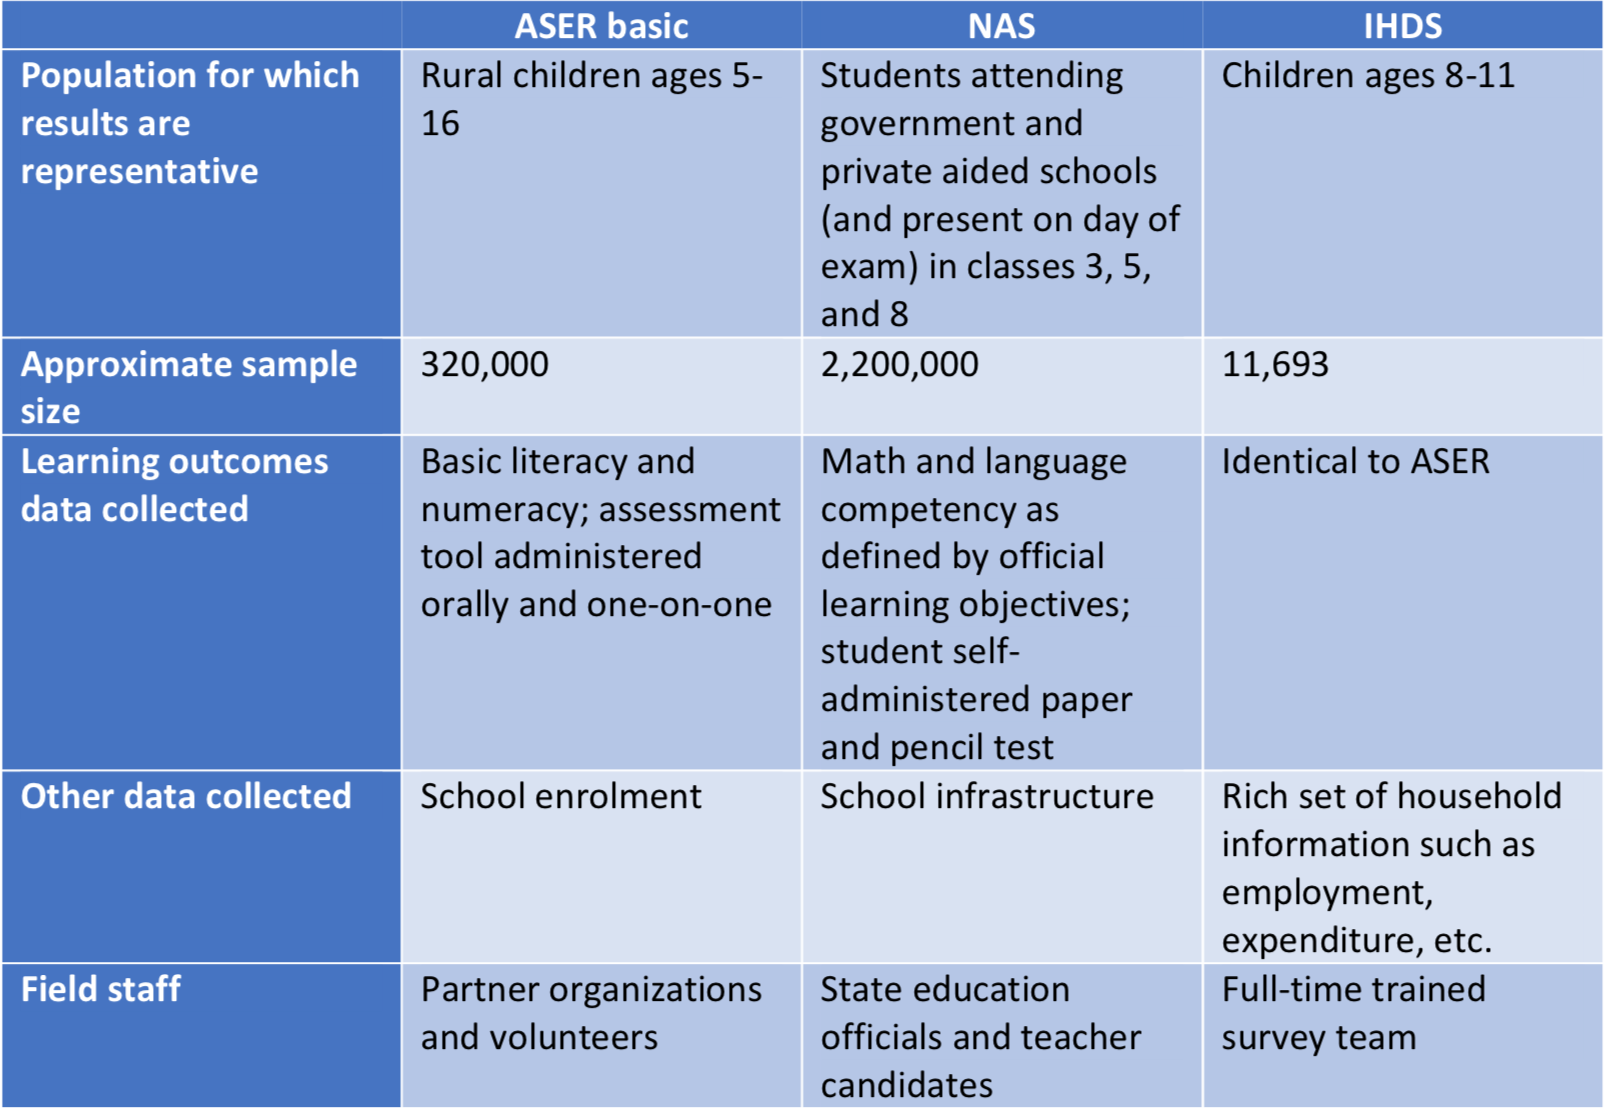
\includegraphics[width=0.8\linewidth]{summary_learning_outcomes} 

}

\caption{Summary of Learning Outcome Surveys}\label{fig:learningoutcomes}
\end{figure}

\hypertarget{comparison}{%
\section{Comparison of ASER, NAS, and IHDS}\label{comparison}}

Direct comparisons of overall results from IHDS, ASER and NAS are not valid as the surveys are representative of different populations and NAS uses a different tool to assess learning outcomes. To facilitate comparison between the three different datasets, we restrict the sample of each of the datasets in several ways to ensure that the state averages from the final three restricted datasets are as similar as possible.

NAS gathers data on whether children attending government or private aided schools in grades 3, 5, and 8 have achieved learning objectives appropriate to their grade level in reading and math. ASER and IHDS gather data on whether rural children of ages 5 to 16 are able to read up to a standard 2 level text and whether they are able to perform math up to division.

We first restrict our focus to reading outcomes. The highest level of the ASER reading assessment corresponds to a standard 2 level text which clearly corresponds to standard 2 level reading proficiency. By contrast, it is more difficult to match the skills tested on the ASER math assessment to NAS grade level objectives. (Recall that NAS does not make public its test questions, only the learning objectives tested.)

Second, we focus on grade 3 students. While ASER assesses older students, comparisons of ASER and NAS for higher grades would not be valid since, for example, NAS assesses 5th grade students on whether they are at a 5th grade reading level while ASER only tests whether 5th grade students have achieved up to a 2nd grade reading level. In theory, this results in a slight discrepancy in the level of learning outcome tested since ASER tests for standard 2 proficiency while NAS tests for standard 3 proficiency. As we will see, NAS scores are actually much higher than ASER for our restricted samples. We include students in grades 2 through 4 in the IHDS sample as otherwise sample sizes per state would be prohibitively small.

Third, we restrict the NAS and IHDS samples to students from rural areas as ASER is only administered in rural areas. Finally, we restrict the three samples to ensure similarity in the types of schools covered. NAS is only administered in government and private aided schools. Unfortunately, we are not able to distinguish between students attending private and private aided schools in the ASER dataset so we restrict the sample to students attending government schools. We include both government and private aided schools in the IHDS sample.

\begin{figure}

{\centering 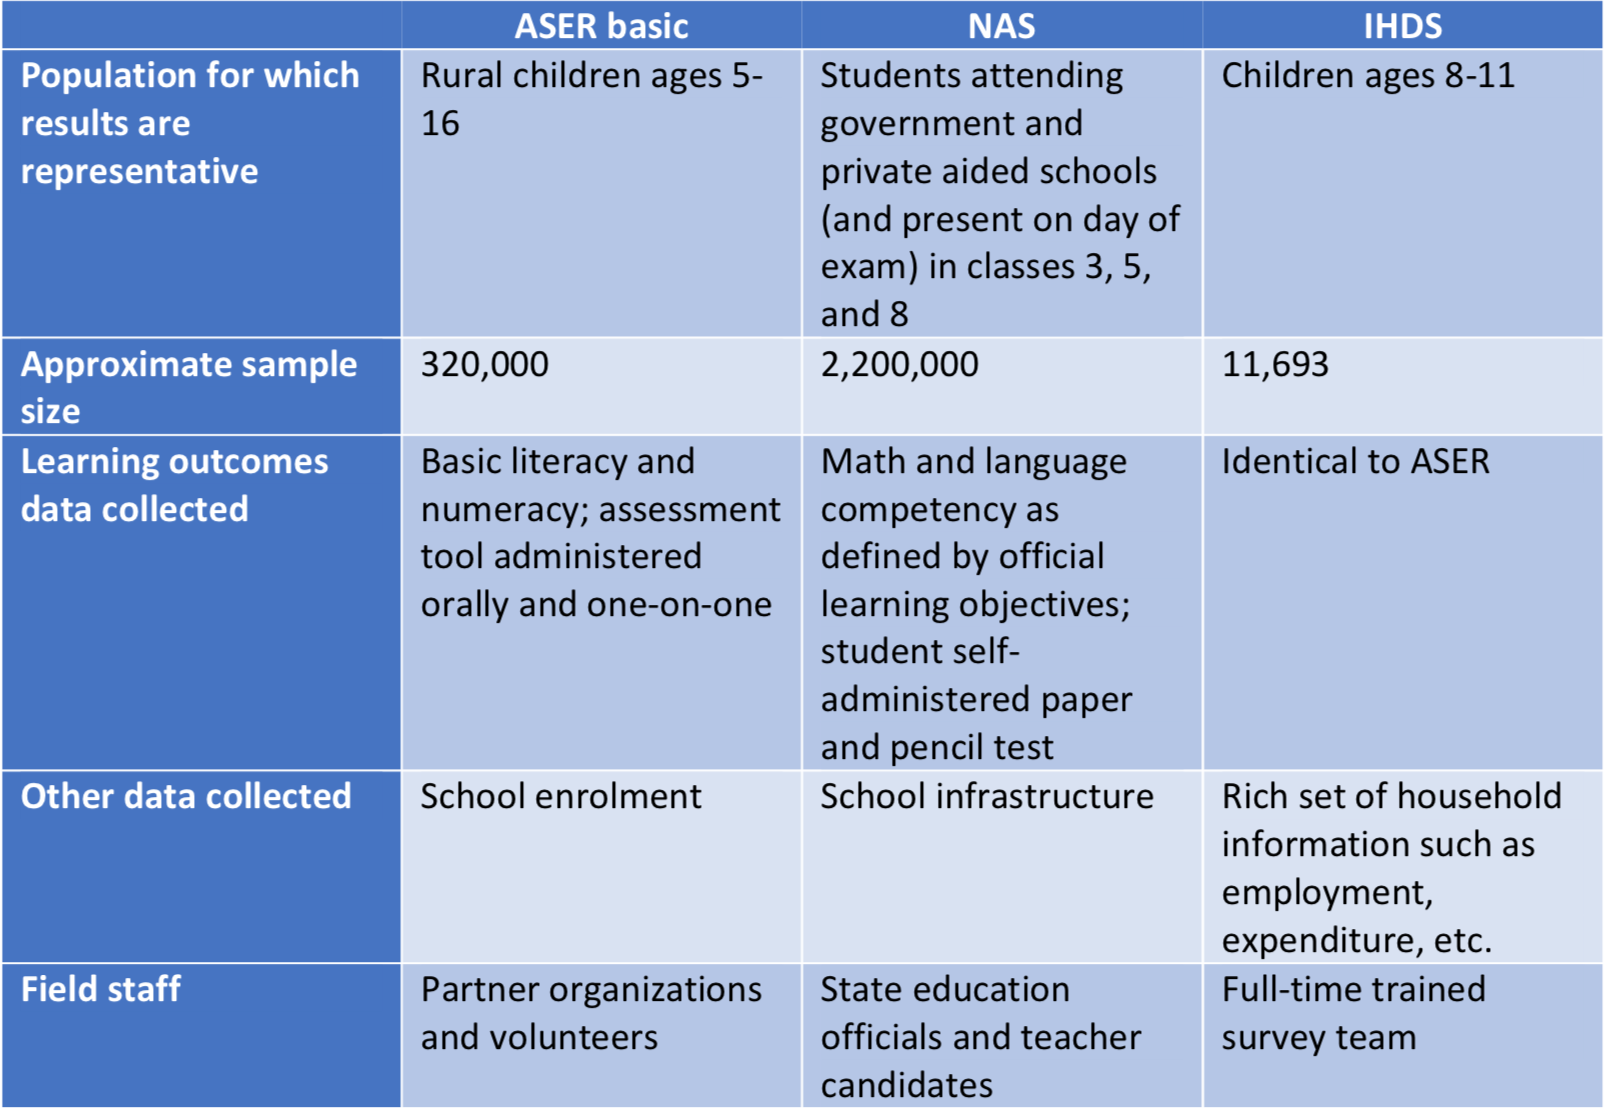
\includegraphics[width=0.8\linewidth]{summary_learning_outcomes} 

}

\caption{Summary of Restricted Samples Used for Comparison}\label{fig:restrictedsample}
\end{figure}

While these restrictions help ensure that the final analytical samples are as comparable as possible, they do not guarantee that the assessment tools are measuring the same latent trait or that the final samples are representative of the same population.

To better understand whether differences in the assessment tools may be driving differences in state averages between the datasets, we compare the correlation between state average NAS and ASER reading scores to the correlation between state average ASER reading and math scores (calculated by taking the correlation between scores in each year and averaging these correlations.) We interpret the correlation between ASER reading and math scores as a crude lower bound of the correlation between ASER state averages and any other well-designed basic reading assessment administered to the same sample of children. While different assessments of basic reading may measure slightly different latent reading abilities, we would expect these latent basic reading abilities to be more highly correlated than basic reading and basic math. Further, previous research has shown that ASER performs well in measuring basic reading ability (Vagh \protect\hyperlink{ref-vagh2012validating}{2012}). If we find the correlation between ASER and NAS state averages is significantly lower than the correlation between ASER state reading and math, we can infer that either a) sampling or survey error is causing differences between the datasets or b) NAS does not accurately measure basic reading ability.

In addition to differences between the assessment tools, differences in the sampling strategy may also drive differences between the datasets. In particular, since NAS is administered in school while ASER is administered at home, any state-level differences in the probability of low/high performing students showing up on NAS exam day would result in differences in the state averages for the two datasets. Of course, if the goal of the NAS survey is to obtain an accurate estimate of learning for all government school students we should still be concerned if we find that differences in test attendance drive differences in results. Nevertheless, understanding whether differences in test attendance may be driving differences in results may be helpful in diagnosing any potential discrepancies between the datasets.

To test whether voluntary student absence on NAS exam day may be driving differences between the datasets we use self-reported data on school attendance from IHDS. Formally, we assume that
the probability of attendance on NAS exam date is \(\frac{30-DAYS_{i}}{30}\) where \(DAYS_{i}\) is the self-reported number of days child i was absent from school in the previous month and calculate expected NAS score taking into account probability of attendance. We caution that these results are only suggestive due to potential measurement error in this variable. In addition, this test only assesses the potential contribution of voluntary student absence. Teachers may have selectively encouraged certain students to stay at home on NAS exam day. \textcolor{red}{Here we should talk about the fact that the IHDS happened in a different year, and why we should not be worried about that}

\hypertarget{results}{%
\section{Results}\label{results}}

Figure \ref{fig:asernasihds} plots class 3 average language scores for rural, government school students from ASER, NAS, and IHDS. IHDS values are missing from some states due to insufficient sample size. Figure \ref{fig:correlations} plots the state rank from ASER on the x axis and the state rank from NAS on the y axis.

\begin{figure}

{\centering 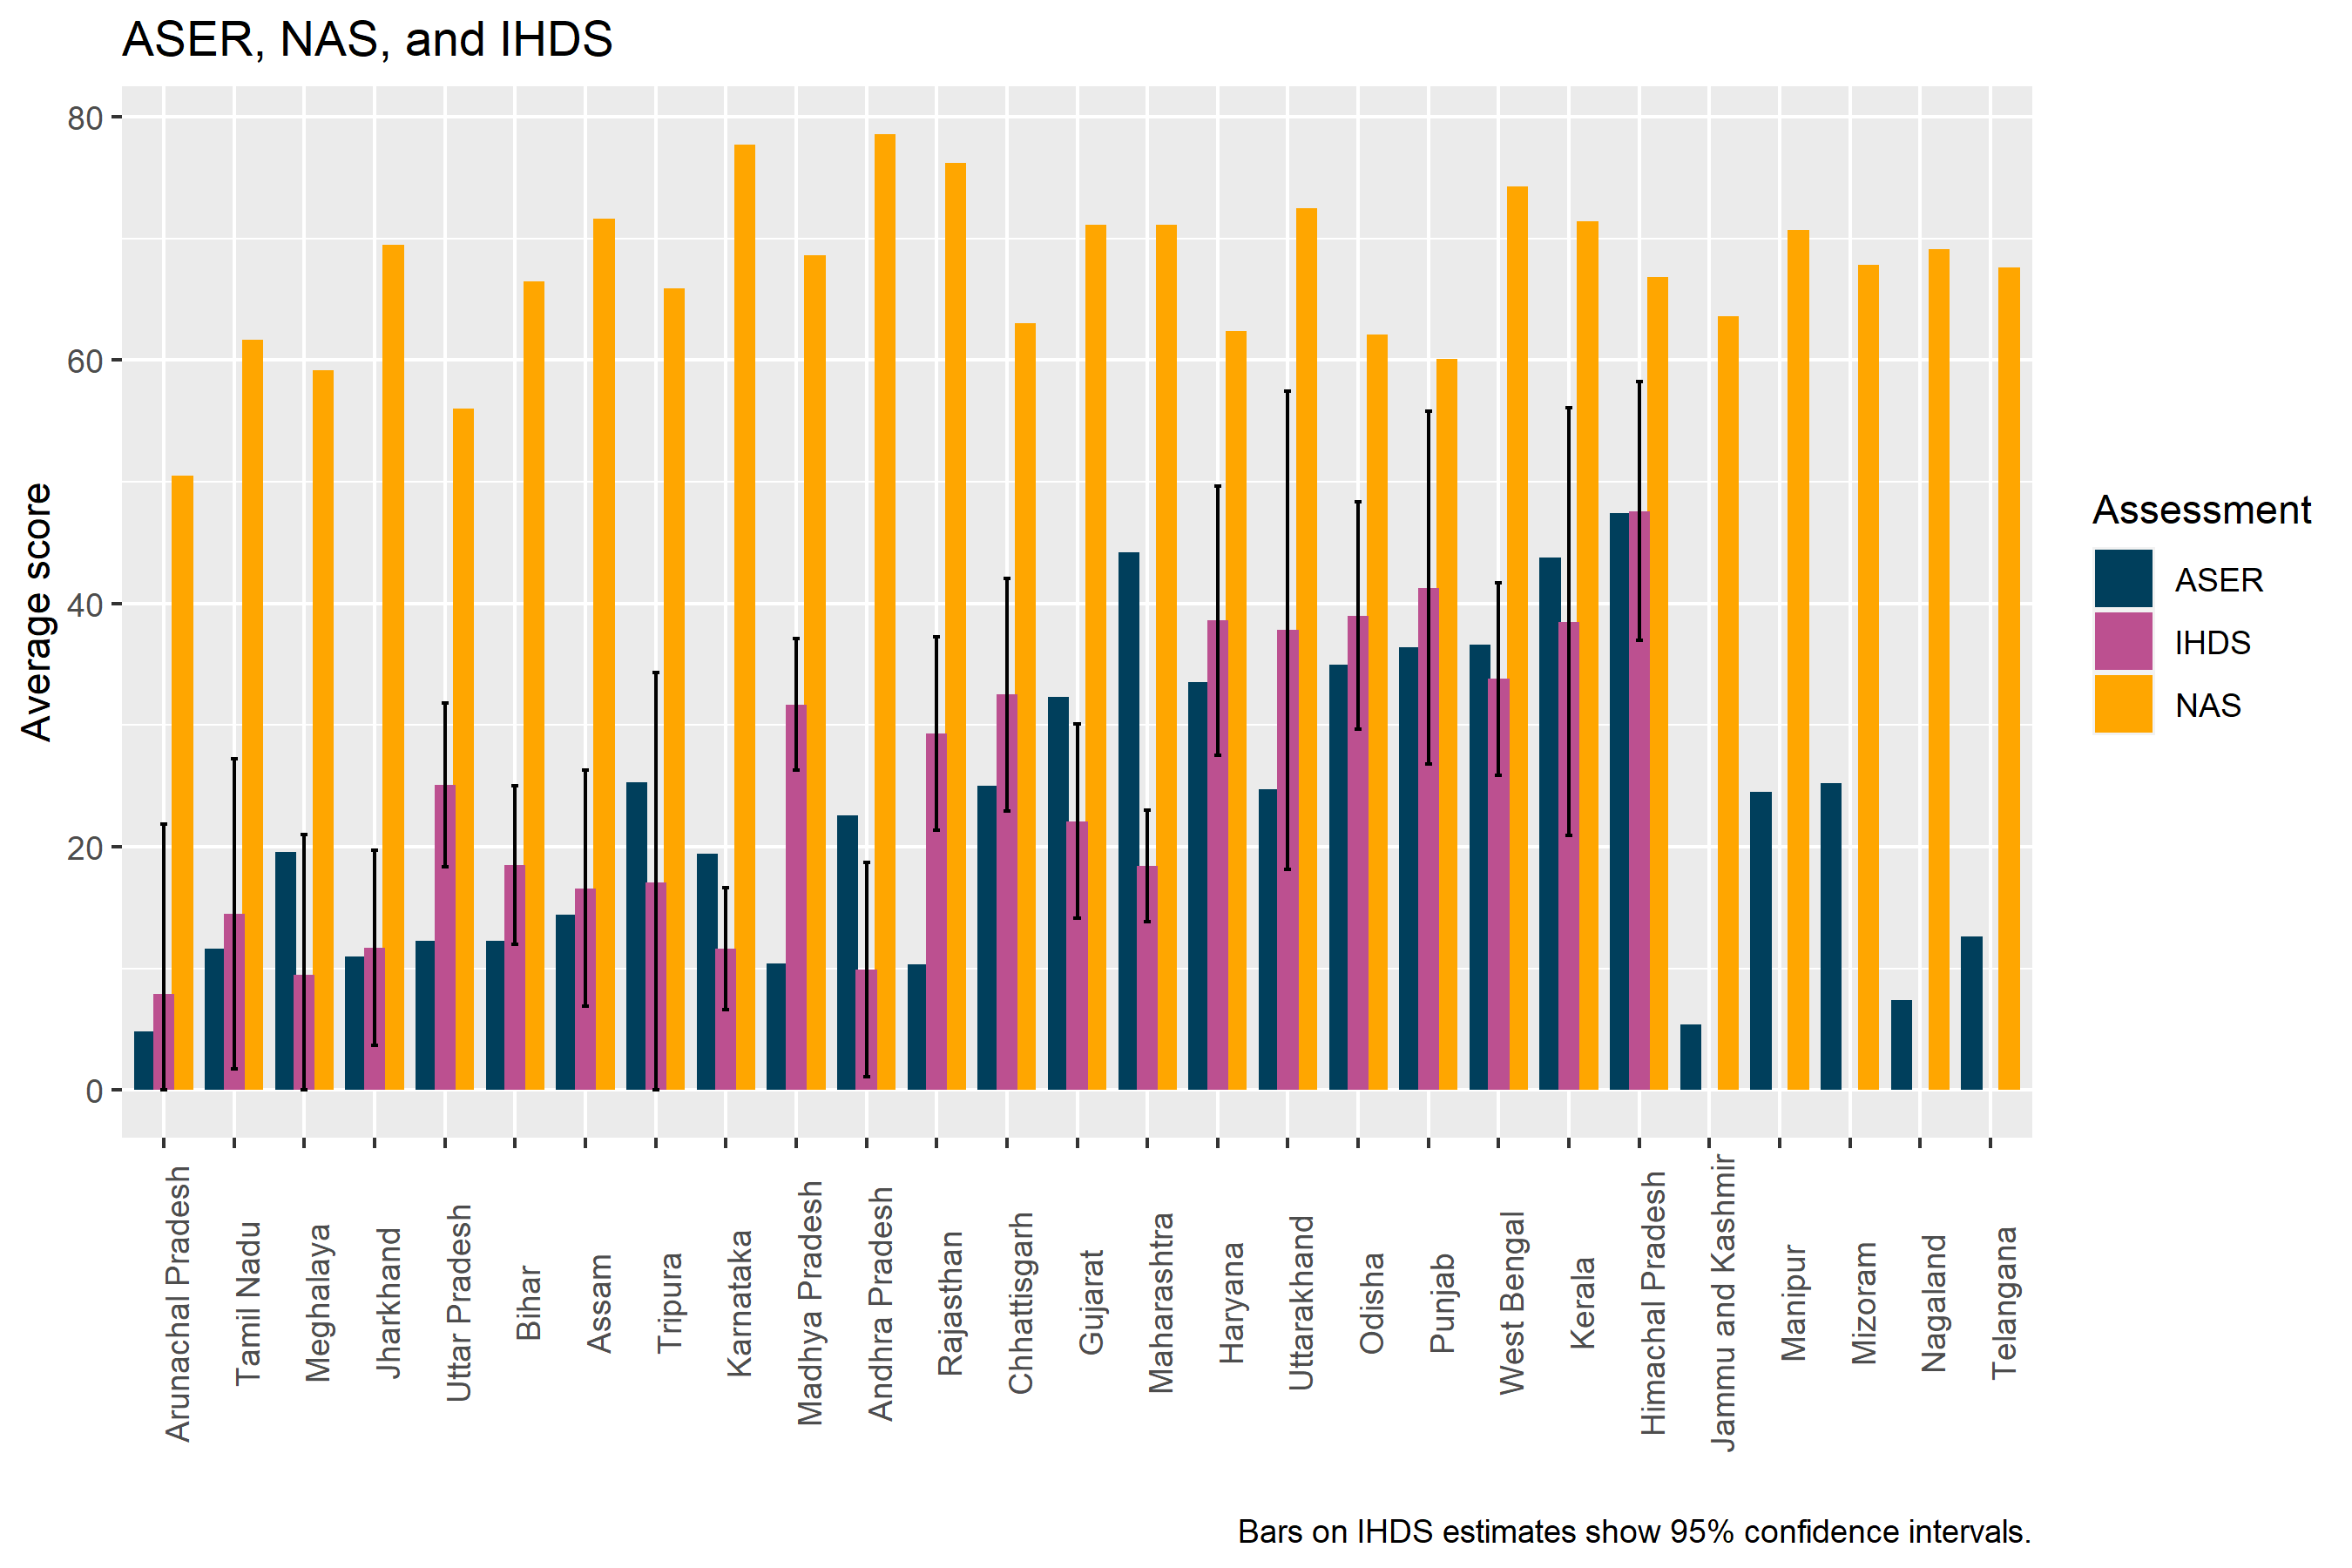
\includegraphics[width=1\linewidth]{aser_nas_ihds_values} 

}

\caption{ASER, NAS, and IHDS}\label{fig:asernasihds}
\end{figure}

\begin{figure}

{\centering 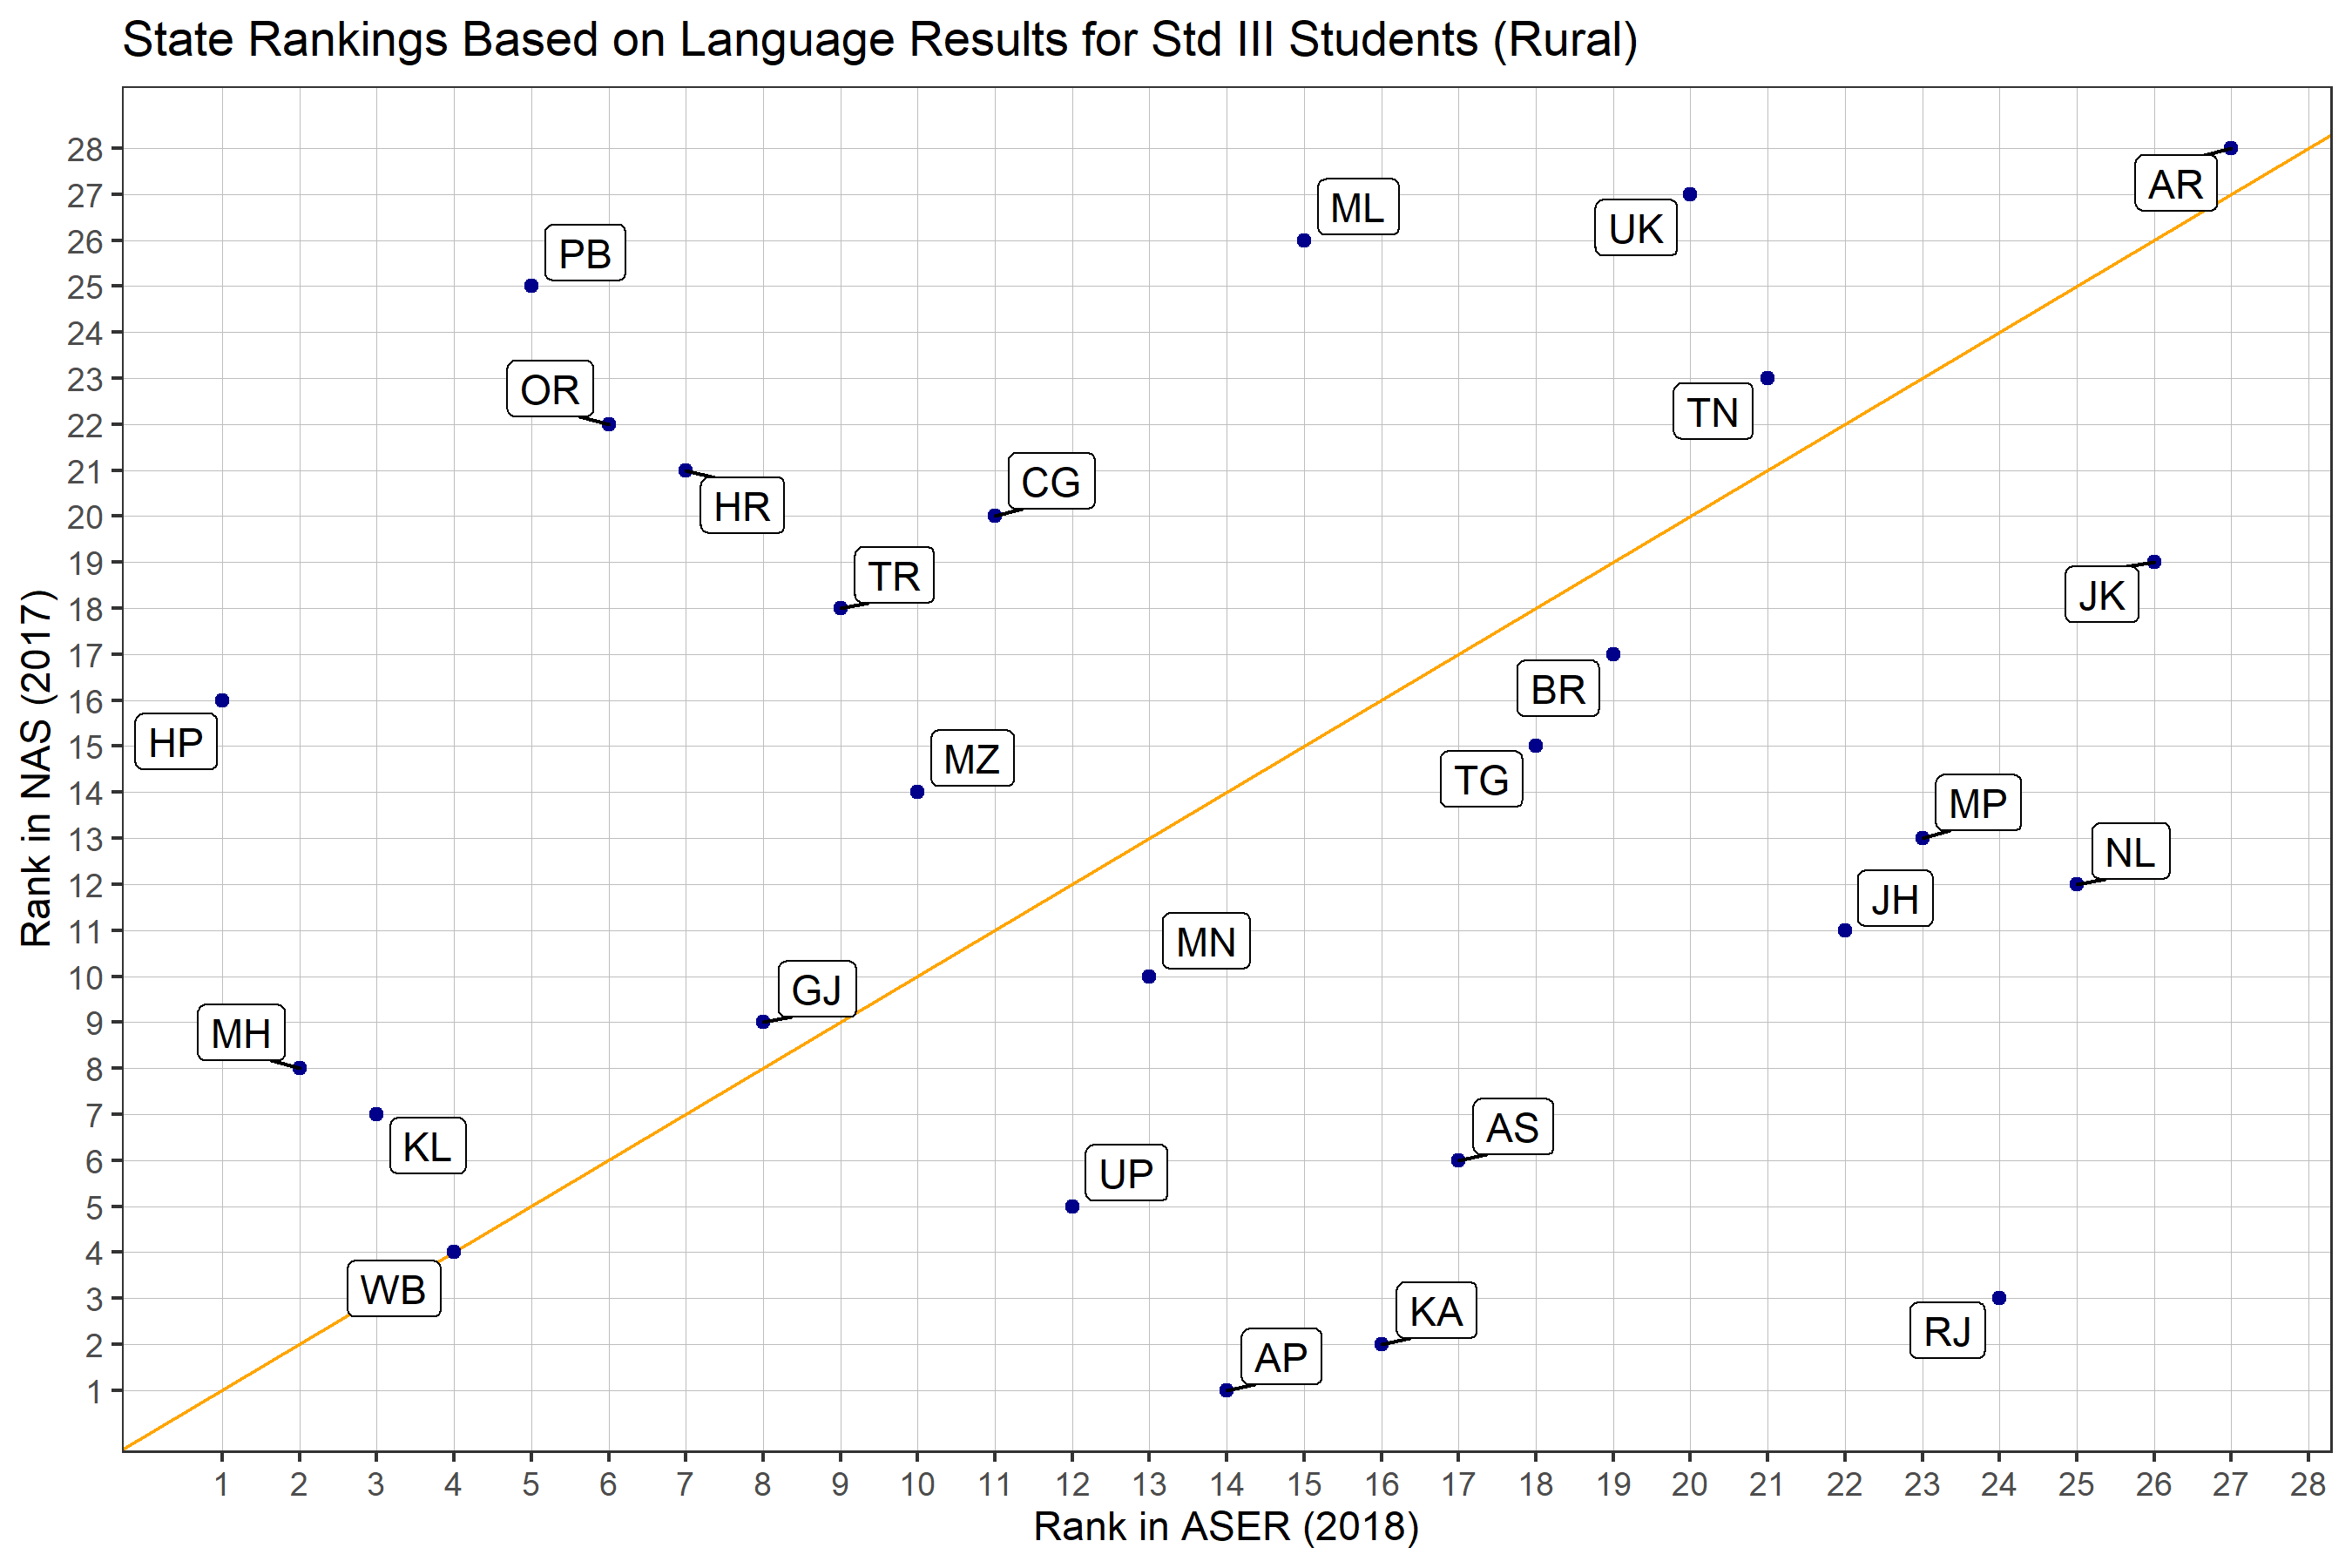
\includegraphics[width=0.8\linewidth]{aser_nas_lang_ranking} 

}

\caption{Correlation Between ASER and NAS}\label{fig:correlations}
\end{figure}

These figures show that IHDS and ASER state averages are very similar in size and that NAS state averages are much higher and not very correlated with either IHDS or ASER. A formal test for correlation confirms that IHDS and ASER are highly correlated (r = 0.62), and NAS is not at all correlated with IHDS (r = -0.03) and only modestly correlated with ASER (r= 0.19). For comparison, ASER grade 3 state average reading and math scores are highly correlated (r = 0.82) suggesting that differences in the aspect of reading being measured likely accounts for very little of this discrepancy.

In addition, comparing ASER and NAS to net state domestic product reveals that ASER is substantially correlated with NSDP (r = 0.41) while NAS is only modestly correlated with NSDP (r = 0.05). (All correlations are Pearson though Spearman gives similar results.) \textcolor{red}{Why do we care about correlating this with NSDP? We should write about that here and maybe cite other work that has done that. Also, we could add in the appendix the results of the Pearman correlation}

Figure \ref{fig:weighted} plots state averages from IHDS taking absence into account (y axis) against state averages when absence is not considered (x axis). Most points in the figure lie slightly above the line of equality, revealing that students with higher rates of absence tend to have lower learning outcomes. However, the effect of these absences on overall scores is very small. In only a few cases does taking absence into account shift relative ranking of the state. (Results available on request.) \textcolor{red}{We should either include these results (here or in the appendix) or not mention this bit if it's not important}

\begin{figure}

{\centering 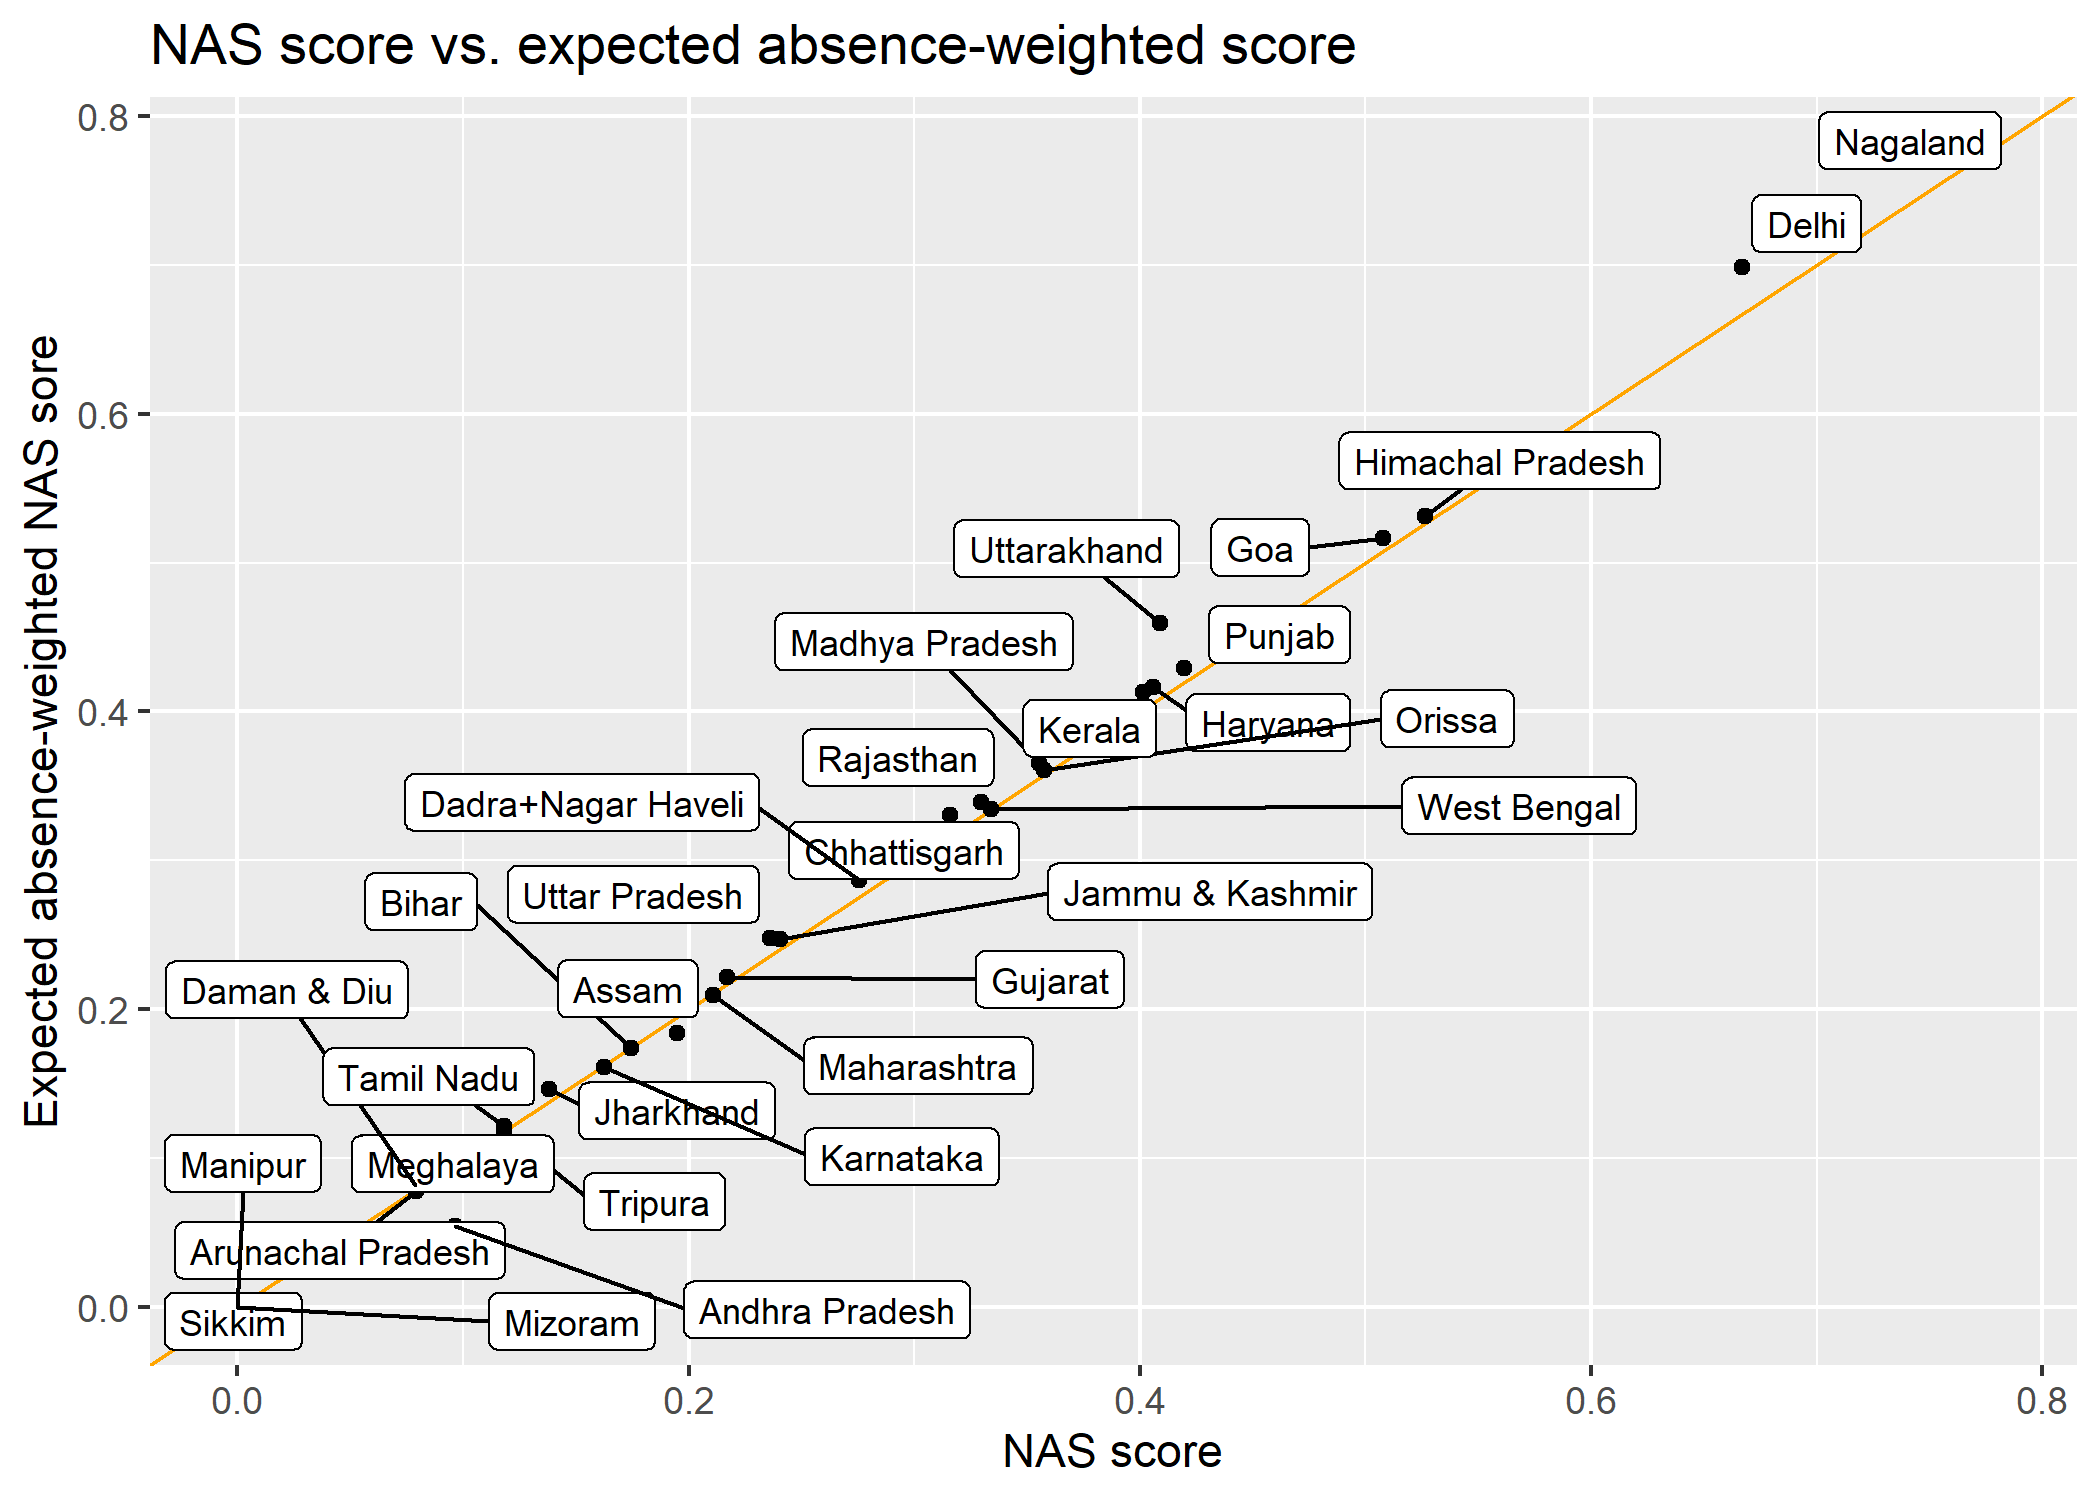
\includegraphics[width=0.8\linewidth]{absence_weighted_aser} 

}

\caption{NAS Score vs. Expected Absence Weighted Score}\label{fig:weighted}
\end{figure}

\hypertarget{aserinternal}{%
\section{Assessing ASER's Reliability}\label{aserinternal}}

\hypertarget{overview-of-approach}{%
\subsection{Overview of Approach}\label{overview-of-approach}}

Similarity between ASER and IHDS data provides reassurance in the reliability of ASER state rankings. Yet ASER's reliance on partner organizations for surveying and the right-hand rule for sampling households generates potential for significant non-sampling errors. This could be the case if, for example, enumerators of a partner organization are slightly more lenient in how they mark the assessment or slightly more likely to survey children who are at home at the time of the survey (as opposed to children determined by the right hand rule).

We analyse the reliability of both ASER scores (i.e.~levels) and changes in ASER scores at the state and district level using two approaches adapted from Kane and Staiger (\protect\hyperlink{ref-kane2002promise}{2002})'s analysis of average school test scores in the US. Kane and Staiger decompose the variance of school average test scores into persistent and transitory components and then further decompose the transitory component into sampling variance and non-sampling variance. Intuitively, this approach looks at whether changes in ASER scores from one round to the next are typically reversed. If changes in scores tend to ``stick,'' we can be relatively confident that the measured change reflects an actual change in underlying learning outcomes. On the other hand, if changes are typically reversed, we would suspect that the measured change was either due to measurement error or some temporary effect on learning outcomes.

The key assumption underlying this approach is that changes in measured scores which persist reflect true changes in learning outcomes while transitory changes are due to noise. True transitory effects on learning outcomes may arise from two main sources. First, some policy or intervention may cause a temporary increase / decrease in learning outcomes which is reversed in subsequent years. Second, one cohort of students may have higher/lower learning outcomes than cohorts above and below. If this is the case, the round in which those students are tested would show higher/lower learning outcomes.

We are unable to test whether temporary increases in learning outcomes are plausible based purely on data but we find it unlikely based on our understanding of education policy in India. Education policies are generally for multiple years and rarely are significant changes rolled back after a single year. By contrast, we are able to empirically test whether differences between cohorts are a likely source of transitory changes in ASER scores by looking at whether changes in grade 3 scores predict changes in grade 5 scores two years later.

\hypertarget{formal-approach}{%
\subsection{Formal Approach}\label{formal-approach}}

We use two different methods to decompose variance into persistent and transitory components.\footnote{Page 247 Kane et al. (\protect\hyperlink{ref-kane2002volatility}{2002}) provides an in-depth derivation of the formula for this first approach. We omit the derivation for the sake of simplicity.} The first method assumes that average test scores \(y_{t}\) for a state or district at time \({t}\) consist of a fixed component \(\alpha\), a persistent component \(v_{t}\) which follows a random walk, and a transitory component \(\epsilon_{i}\) which is i.i.d. so that average test scores equal:

\[ 
\begin{aligned}
y_{t} &= \alpha + v_{t} + \epsilon_{t} \\
where \; v_{t} &= v_{t-1} + u_{t}
\end{aligned}
\]

Then, \(Var(\Delta y_{t}) = \sigma^2_{u} + 2\sigma^2_{e}\) and the proportion of the overall variance of the changes in \(y\) arising due to the transitory shock can be estimated as:
\[
\begin{aligned}
  -2*corr(\Delta y_{t}, \Delta y_{t-1}) &= 
  -2*corr(u_{t} + \epsilon_{t} - \epsilon_{t-1},u_{t-1} + \epsilon_{t-1} - \epsilon_{t-2}) \\
  &= \frac{2\sigma^2_{e}}{\sigma^2_{u} + 2\sigma^2_{e}}
\end{aligned}
\]
Similarly, we can also estimate the proportion of variance in levels (as opposed to changes) which are due to the transitory shock by rearranging the formula above to get:
\[
\sigma^2_{e} = corr(\Delta y_{t}, \Delta y_{t-1}) *Var(\Delta y_{t})
\]

A potential downside to this method is that it relies on the assumption that the \(u_{t}\) and \(\epsilon_{t}\) terms are not serially correlated. The \(u_{t}\) terms may be serially correlated if, for example, states or districts often implement programs which result in not just one-off increases (decreases) in learning outcomes but multi-year increases (decreases) in learning outcomes. Similarly, the \(\epsilon_{t}\) terms may be serially correlated if partner organizations collect data in the same areas for multiple years. Positive auto-correlation in either \(u_{t}\) or \(\epsilon_{t}\) terms will bias downwards our estimate of the proportion of variance due to transitory shocks.

We can partially test for this by looking at \(corr(\Delta y_{t}, \Delta y_{t-2})\). If the \(u_{t}\) and \(\epsilon_{t}\) terms are not serially correlated, the correlation in current changes and twice lagged changes should be 0 (though this correlation may also equal 0 under other conditions as well)\textcolor{red}{What conditions where you thinking about? Should we add something about this as a footnote?}. We find that this holds approximately for district changes (correlation with double lag is 0.04 for reading and -0.04 for math) but not for the state changes (the correlation with double lag ranges from 0.1 to 0.18). Thus, for states we also use a second method for decomposing variance into persistent and transitory components developed by Kane and Staiger. We focus on results from this second method in the main results section but also present results from the first method in figure \ref{fig:variance} in the appendix. Results from the first method do not alter our substantive results.

The second method relies on the fact that if there is both a persistent component and a transitory component to scores, we would expect the correlation between current scores and the first lagged score to reflect both persistent and transitory shocks while the correlation between current scores and further lags would mainly reflect the persistent component. Thus, when comparing correlation between current scores and previous scores for increasing lags, the correlation should fall quite a bit with the first lag and then exhibit relatively steady decay after that. The figure below shows the average correlation between current state averages and previous state averages for lags up to five years. For both reading and math, the initial decrease in correlation (starting from 1) is larger than the subsequent decreases and subsequent decreases tend to be relatively stable.

\begin{figure}

{\centering 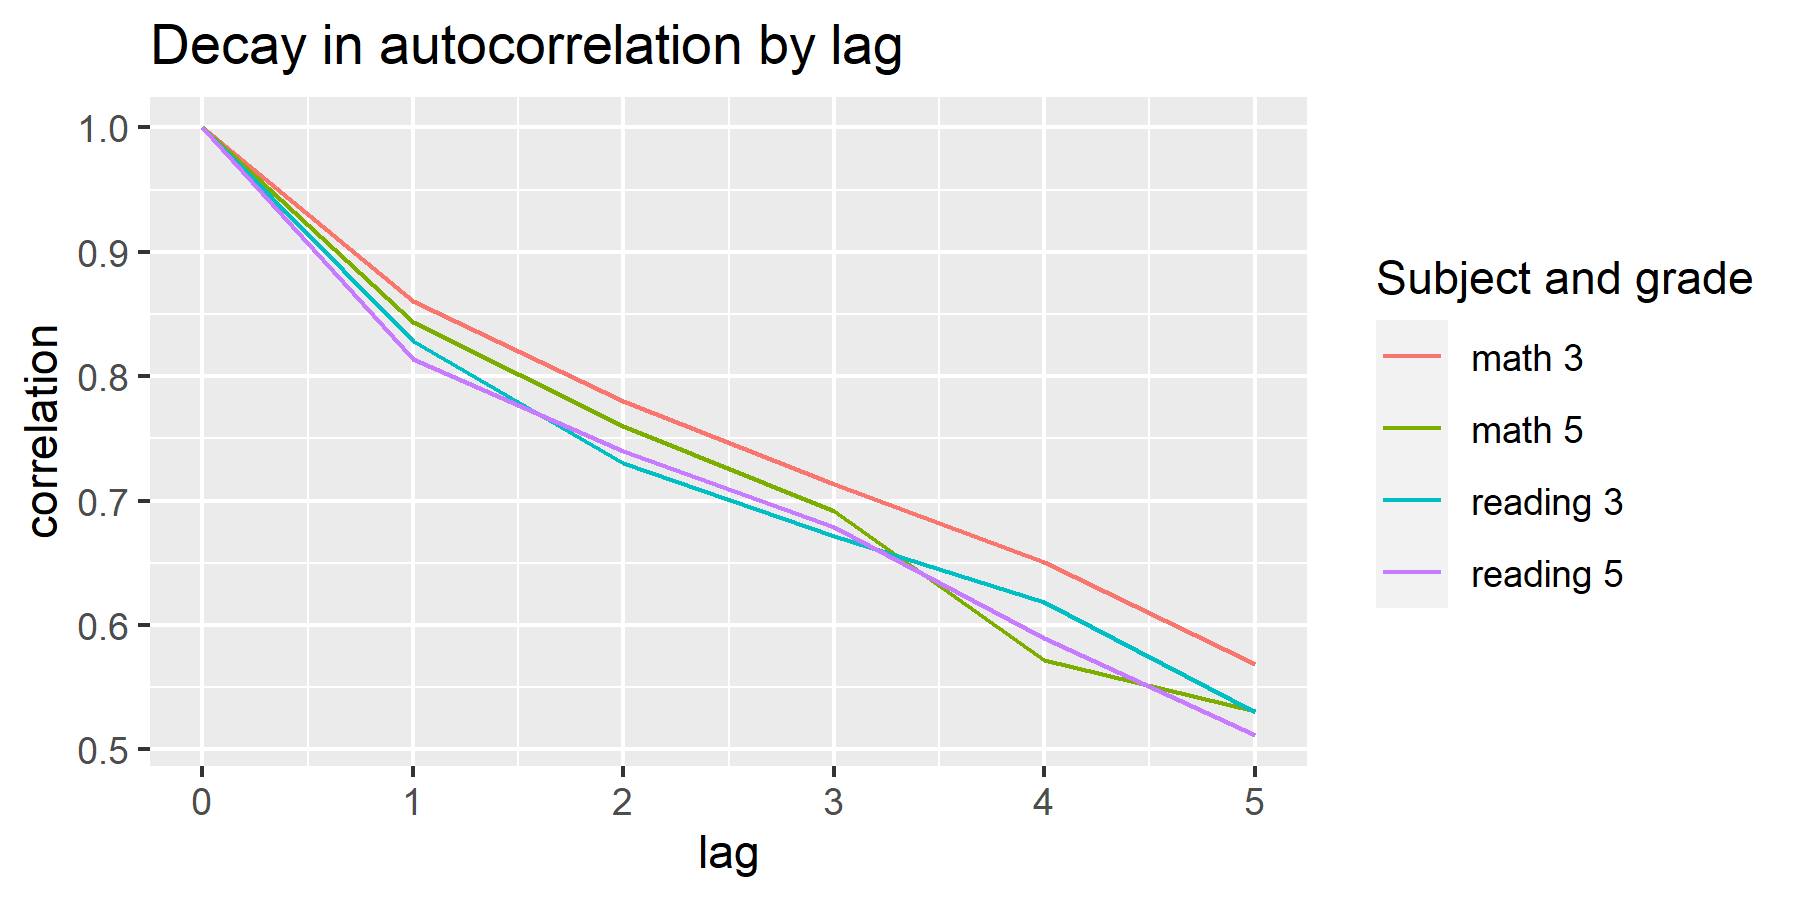
\includegraphics[width=0.8\linewidth]{Correlation decay} 

}

\caption{Autocorrelation Decay}\label{fig:decay}
\end{figure}

Using this method, we can then estimate the variance of the persistent component, \(\sigma^2_{pers}\), using the correlation of current scores with the kth lag, \(\rho_{k}\):

\[
\begin{aligned}
  \sigma^2_{pers} &= 1 - \sigma^2_{\epsilon} \\
  &\approx \frac{\sigma^2_{y}\rho}{\rho_{pers}} \\
  where \; \rho_{pers}  &\approx K^{-1}\sum_{k=1}^4\frac{\rho_{k+1}}{\rho_k}
\end{aligned}
\]

Once we have calculated \(\sigma^2_{pers}\) and \(\sigma^2_{sampling}\) (see below) we calculate the variance of non-sampling transitory effects as the residual, \(\sigma^2_{other} = \sigma^2_{y} - \sigma^2_{pers} - \sigma^2_{sampling}\). For changes in state scores, we calculate the persistent effects as \(\sigma^2_{pers,changes} = \sigma^2_{\Delta y}-2*\sigma^2_{other}-2*\sigma^2_{sampling}\).

For both methods, we decompose \(\sigma^2_{\epsilon}\) into variance arising from sampling and variance arising from other transitory effects using analytical estimates of sampling variance. ASER doesn't publish standard errors and we don't have access to the microdata so we are unable to directly estimate the standard errors. However, we may estimate standard errors using the ASER sampling strategy combined with estimates of sampling parameters from IHDS.

Using IHDS, we find that that the Inter-cluster Correlation Coefficient (ICC) of ASER scores at the village level is around 0.18. Within each district, ASER samples 30 villages and interviews 20 households per village. For a variable with prevalence of 0.5, the sampling variance for district averages is approximately:\footnote{In the interest of simplicity, we don't take into consideration the rotating panel nature of the ASER survey.}\footnote{In line with the survey sampling literature, we refer to the variance arising from fidelity to the intended sampling strategy ``sampling variance.'' Note that this does not include variance arising from potential deviations from the sampling strategy. (For example, if some surveyors selected more easily available households.)} \textcolor{red}{I think we should explain this in a lot more detail. For instance, why do we need the ICC? and what is DEFF? Is that something that is well known in the literature?}

\[
\begin{aligned}
  DEFF = 1 + (20 - 1)*ICC \\
  \sigma^2_{2} = \frac{DEFF*0.5^2}{600} = 0.0018
\end{aligned}
\]

We may compare this estimate with standard errors reported in a technical paper on ASER precision published by the ASER centre (Ramaswami and Wadhwa \protect\hyperlink{ref-ramaswami2010survey}{2010}). Variance of estimates for districts reported in this paper are around 0.0016. The similarity between the two figures lends confidence to our estimates. We take as our final estimate of the variance of district estimates due to sampling as 0.0016, though other similar values don't change our results substantially.

To calculate sampling variance at the state level, we divide this variance by the number of districts in the state and then take the average across states. While this approach is slightly crude, sampling variance at the state level is very small and thus unlikely to affect our results.

The critical assumption underlying this analysis is that transitory shocks to ASER scores are due to noise rather than actual changes in learning outcomes. One potential source of true transitory effects on learning outcomes is differences between cohorts. We may test whether cohort effects account for a substantial share of year to year changes by looking at whether grade 3 changes in scores anticipate grade 5 changes in scores. Shifting perspectives slightly, we can think of ASER scores as composed of three components: the beginning of year learning level for the cohort in that year, the learning gain in that year, and a noise term, i.e.:

\[
\begin{aligned}
 y_{t} &= c_{t, start} + l_{t} + \epsilon_{t} \\
 & = c_{t,end} + \epsilon_t
\end{aligned}
\]
Note that there is no clear mapping between the decomposition of scores above and this new formulation (aside from the fact that the noise term is clearly transitory): both cohort and learning changes may be persistent or transitory. Our goal is not to show that cohort effects are unlikely to be transitory but rather to test for cohort effects at all. If we can rule out cohort effects, we may conclude that transitory effects are unlikely to be due to cohort effects.

We can estimate the variance in changes due to cohort effects by running the following regression:

\[
\begin{aligned}
  \Delta y_{5,t} = \beta\Delta y_{3,t-2} + \epsilon_{t}
\end{aligned}
\]
If \(corr(\Delta \epsilon_{t-2},\Delta \epsilon) = 0\) then \(plim(\beta) = \gamma(\frac{\sigma^2_{\Delta c_{end}}}{\sigma^2_{\Delta c_{end}}+\sigma^2_{\Delta \epsilon}})\) where \(\gamma\) is the coefficient from a regression of \(\Delta c_{5,t,end}\) on \(\Delta c_{3,t,end}\). If \(corr(\Delta c_{3,t-2,end},\Delta c_{3,t-2,end}) = 1\) and \(corr(\Delta c_{3,t-2,end},\Delta l_{4,t-1}+ \Delta l_{5,t}) = 0\) then \(\gamma = 1\) and \(\beta\) serves as an estimate of the share of the variance of the changes in scores due to cohort effects. There are several reasons why these assumptions may not hold. For example, top-coding in the ASER scores may lead to compression of differences or differences in the two learning outcomes measures used in grades 3 and 5 may lead to lower than 1 correlation between the measured cohort differences. We believe these causes are unlikely to seriously affect the value of \(\gamma\) (few state scores are very close to either 0 or 1 and, in most states, absolute values for grade 3 and 5 scores are remarkably similar) but nevertheless consider \(\beta\) a rough approximation of the share of variance in changes due to cohort effects.

The data we use for these analyses differs from that used above to compare ASER and NAS in several respects. First, state and district averages include all students, not just those attending government schools. Second, for districts we use the share of standard 3, 4, and 5 students who can at least read a standard 1 text and can at least perform subtraction. Our district data is from 2006 to 2011. ASER only publishes two variables for district averages (these variables and the share of standard 1 and 2 students who can recognize letters and who can recognize numbers). The variables chosen are closer to the variable used in the analysis above and also more likely to be stable over time due to the inclusion of 3 grade levels. For states, we use the a) share of class 3 children who can at least read a standard 1 text, b) the share of class 3 children who can do at least subtraction, c) the share of class 5 children who can read at least a standard 2 text, and d) the share of class 5 children who can perform simple division. Our state data is from 2006 to 2014. Again, our choice of variables is driven by availability of data. These are the only variables easily accessible for all years in our dataset.

\hypertarget{aser-internal-reliability-results}{%
\subsection{ASER Internal Reliability Results}\label{aser-internal-reliability-results}}

Figures \ref{fig:aserread} and \ref{fig:asermath} display ASER state reading and math scores for grade 3 and 5 over time. The figures show that even at the state level, ASER scores are quite ``jumpy.'' In addition, based on visual inspection it does not appear that grade 5 scores are influenced by lagged grade 3 scores.

\begin{figure}

{\centering 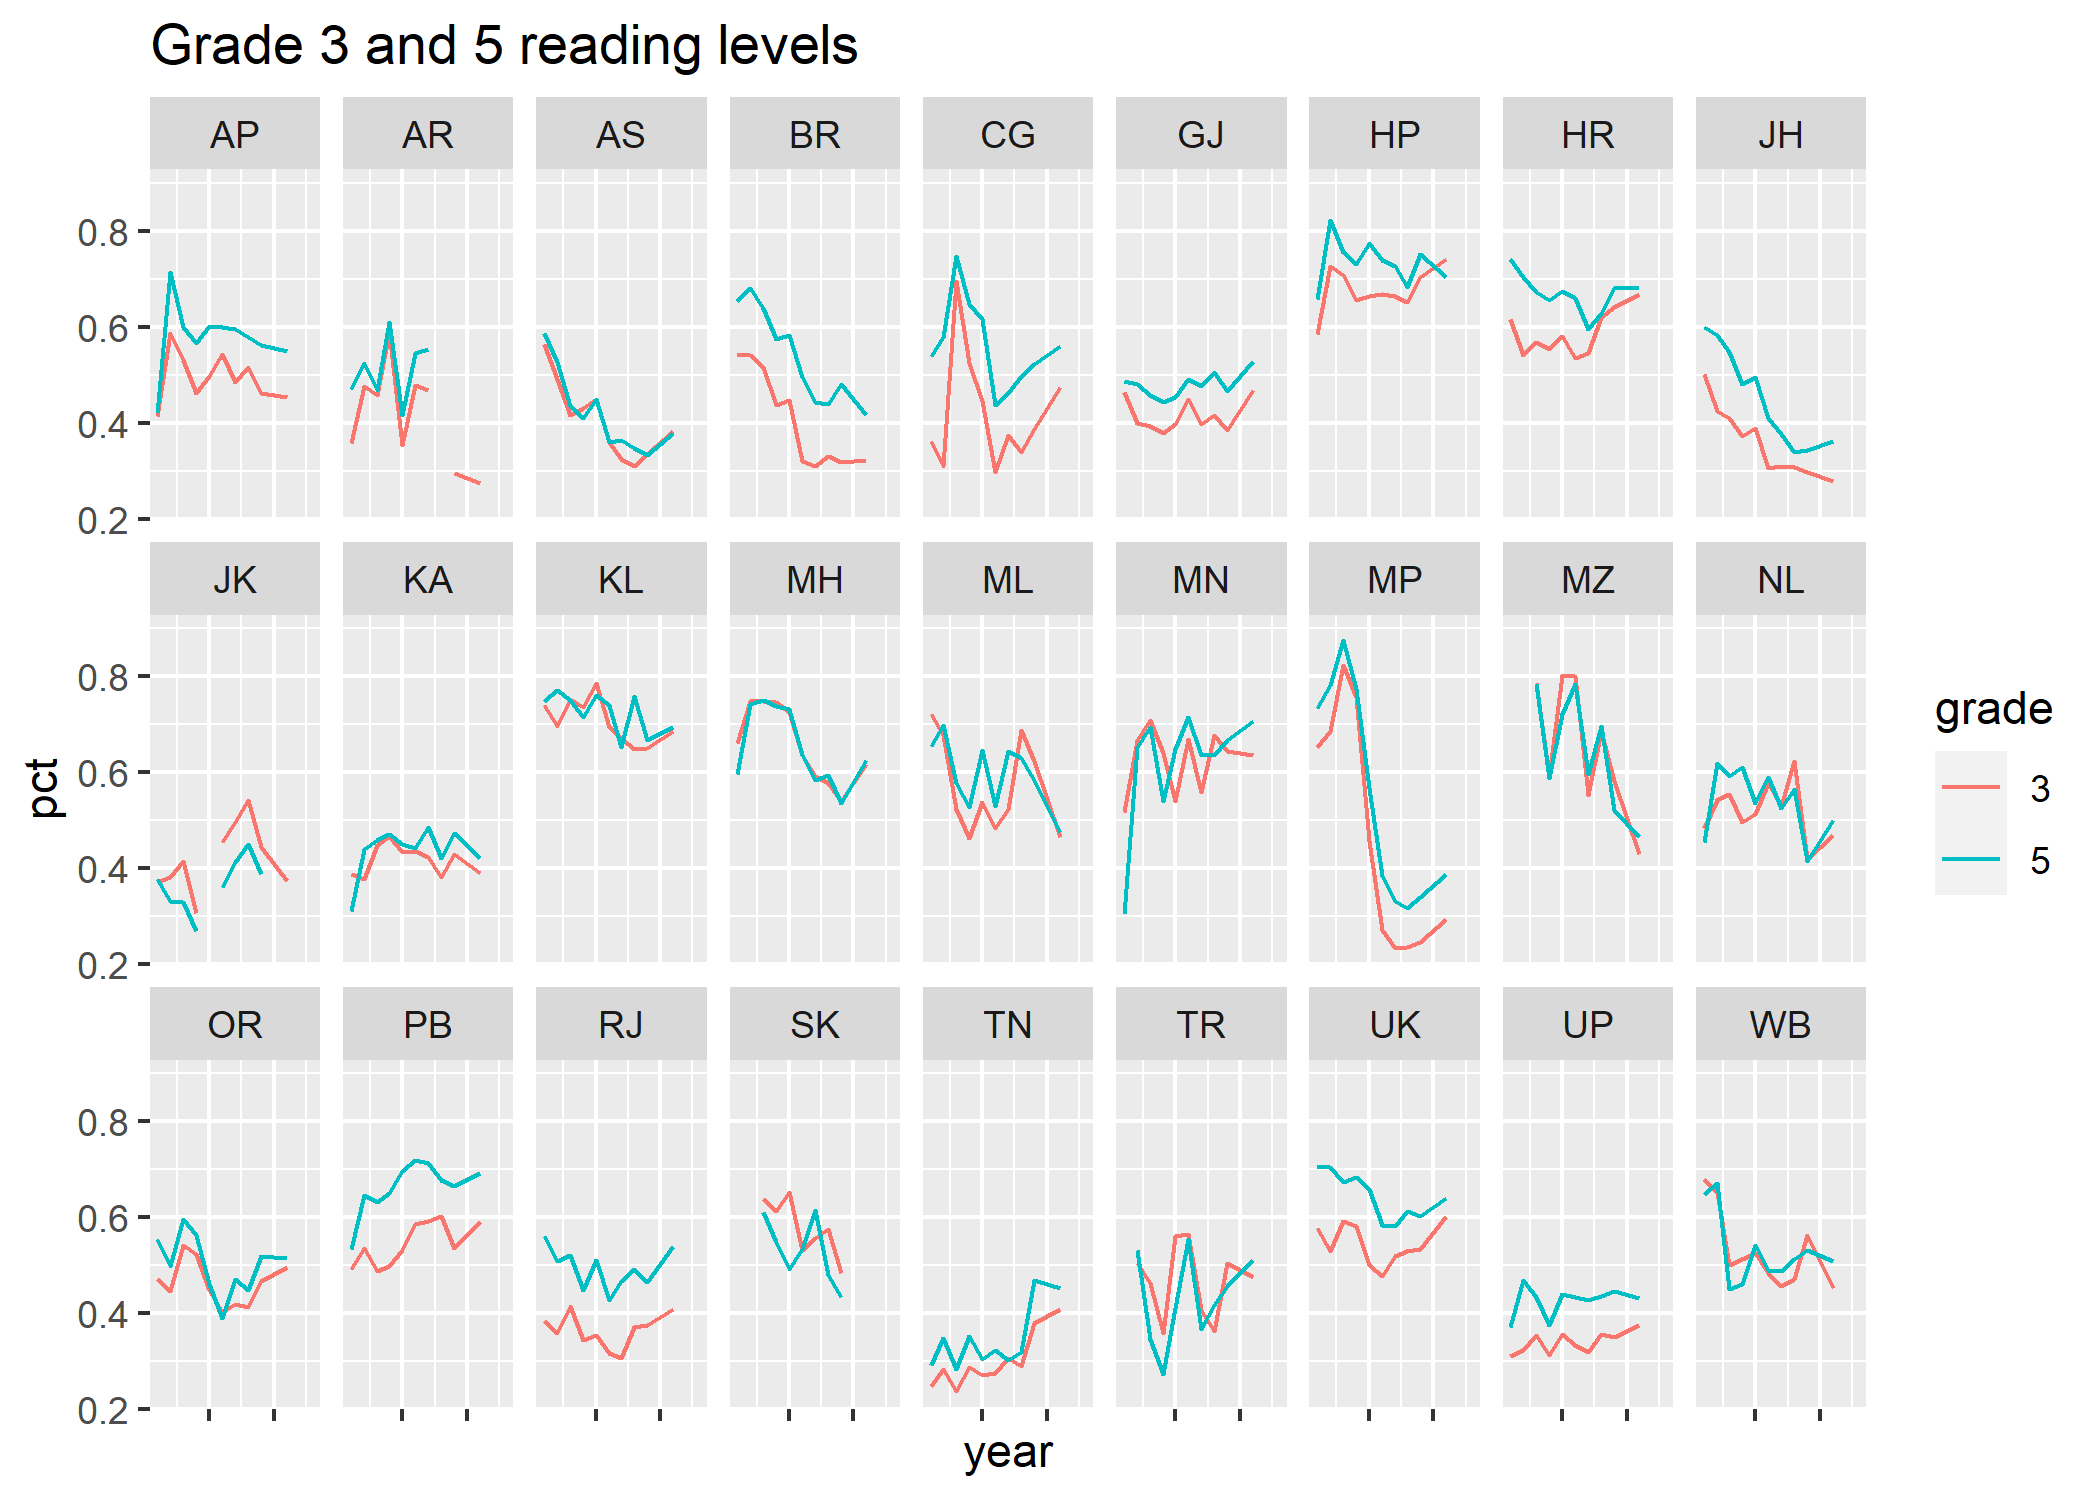
\includegraphics[width=0.8\linewidth]{aser reading over time} 

}

\caption{Reading Levels Over Time}\label{fig:aserread}
\end{figure}

\begin{figure}

{\centering 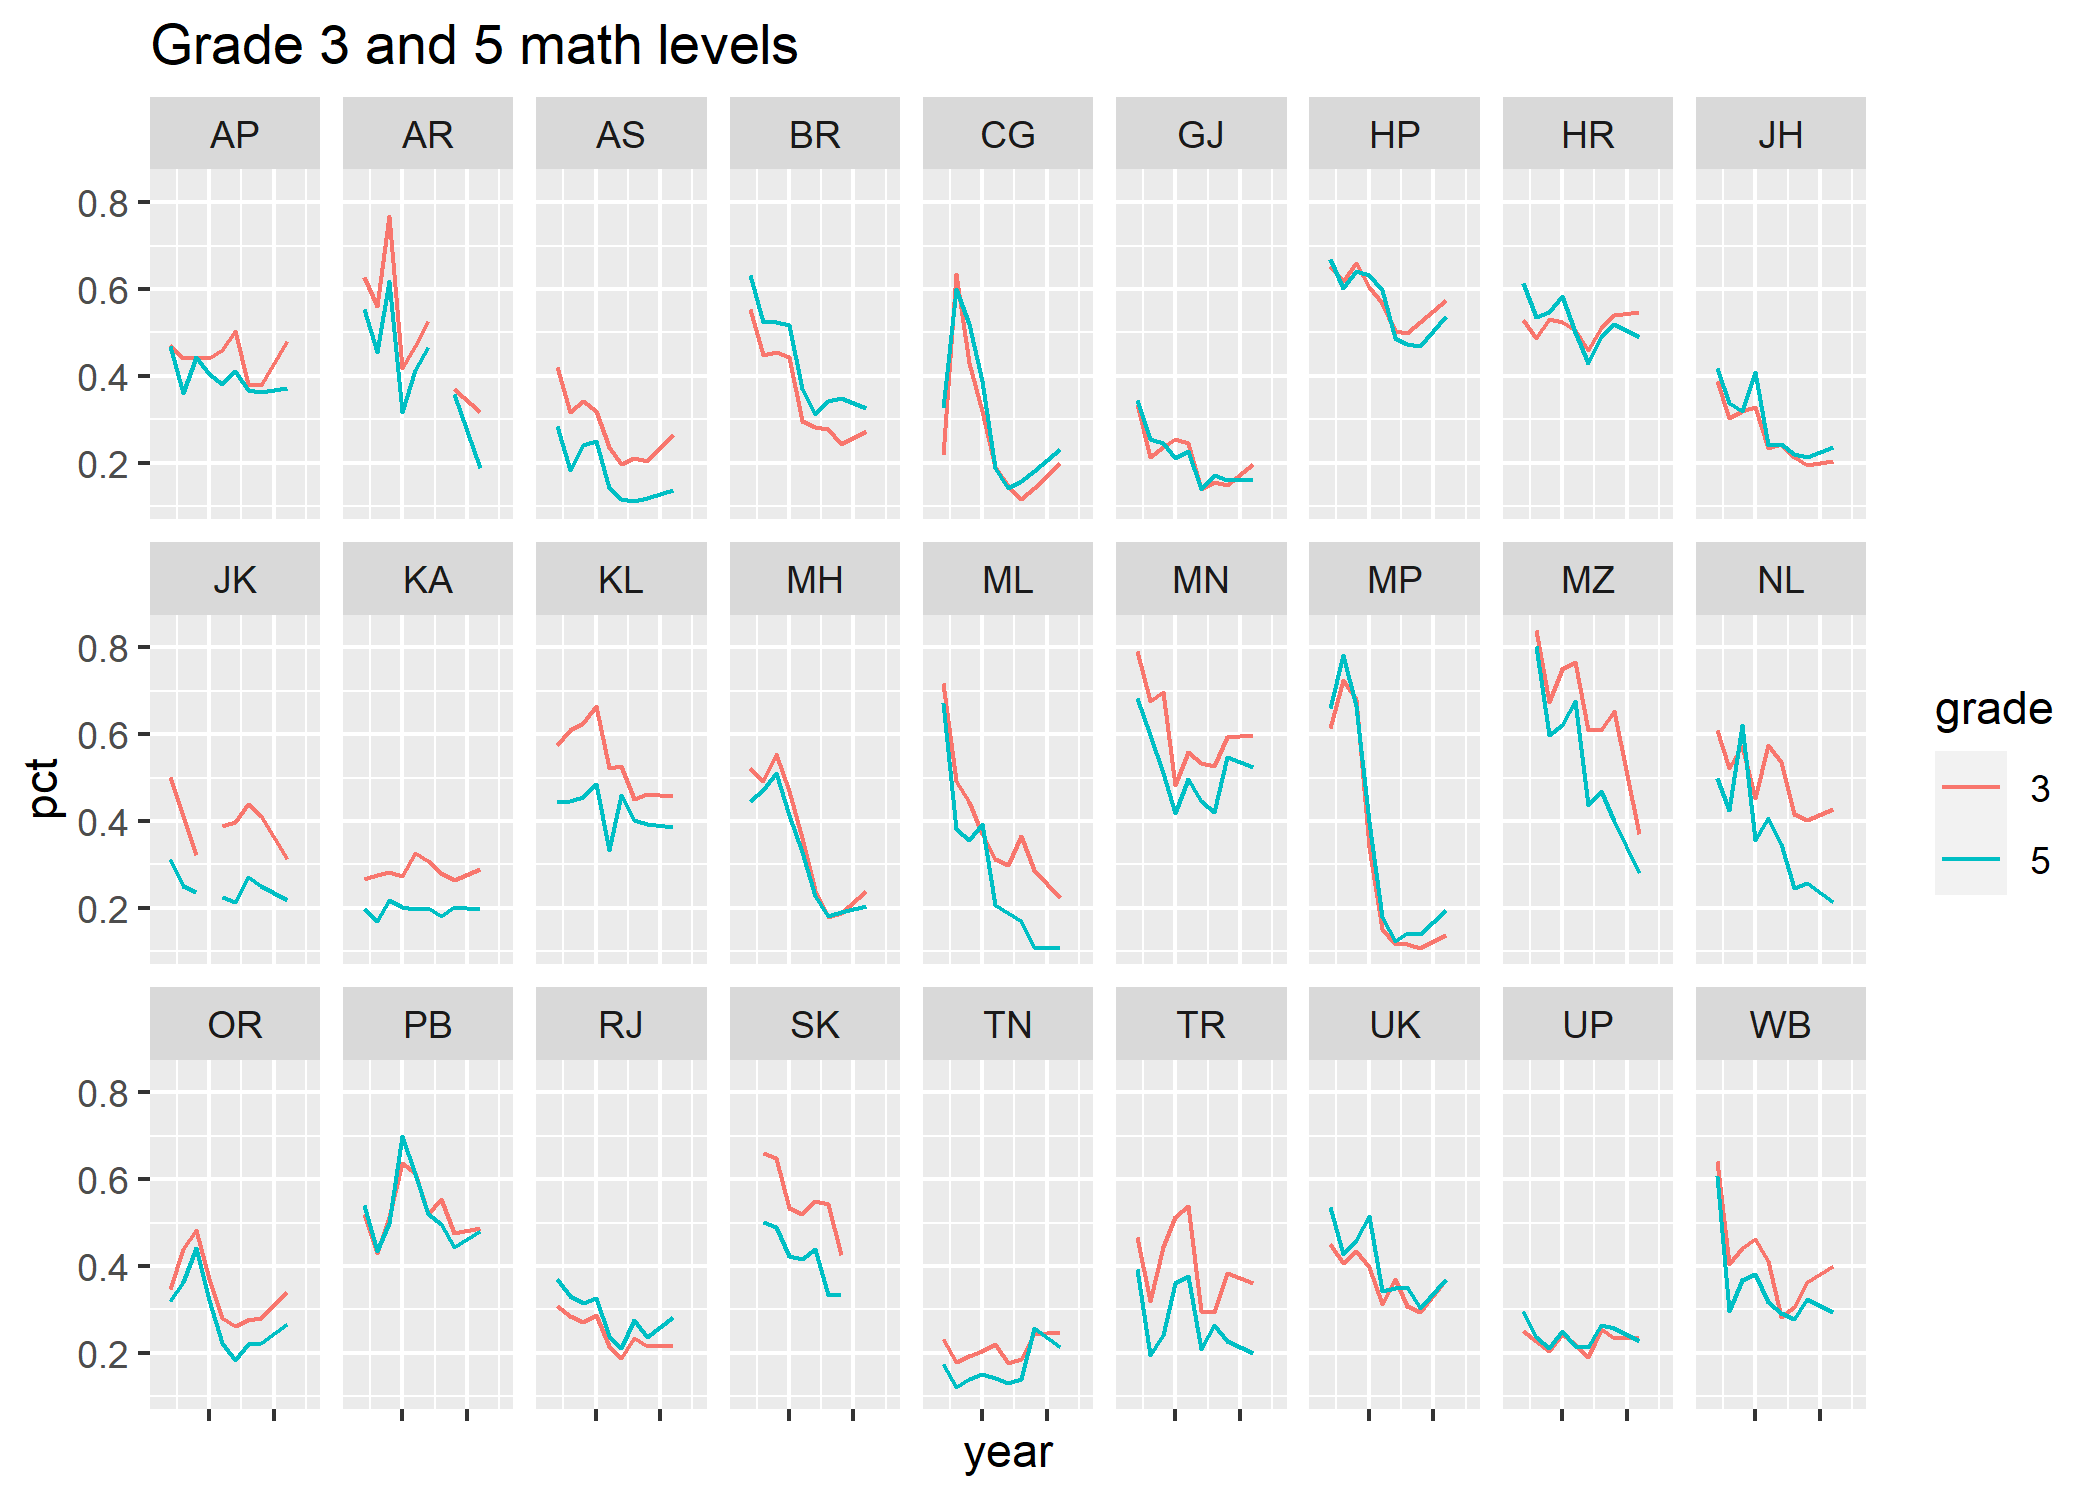
\includegraphics[width=0.8\linewidth]{aser math over time} 

}

\caption{Math Levels Over Time}\label{fig:asermath}
\end{figure}

Figure \ref{fig:combinedbarchart} displays the breakup of variance into a persistent component, sampling, and non-sampling transitory effects. Figure \ref{fig:variance} in the appendix displays the same information but in numerical form and as shares of the total rather than absolute size.

\begin{figure}

{\centering 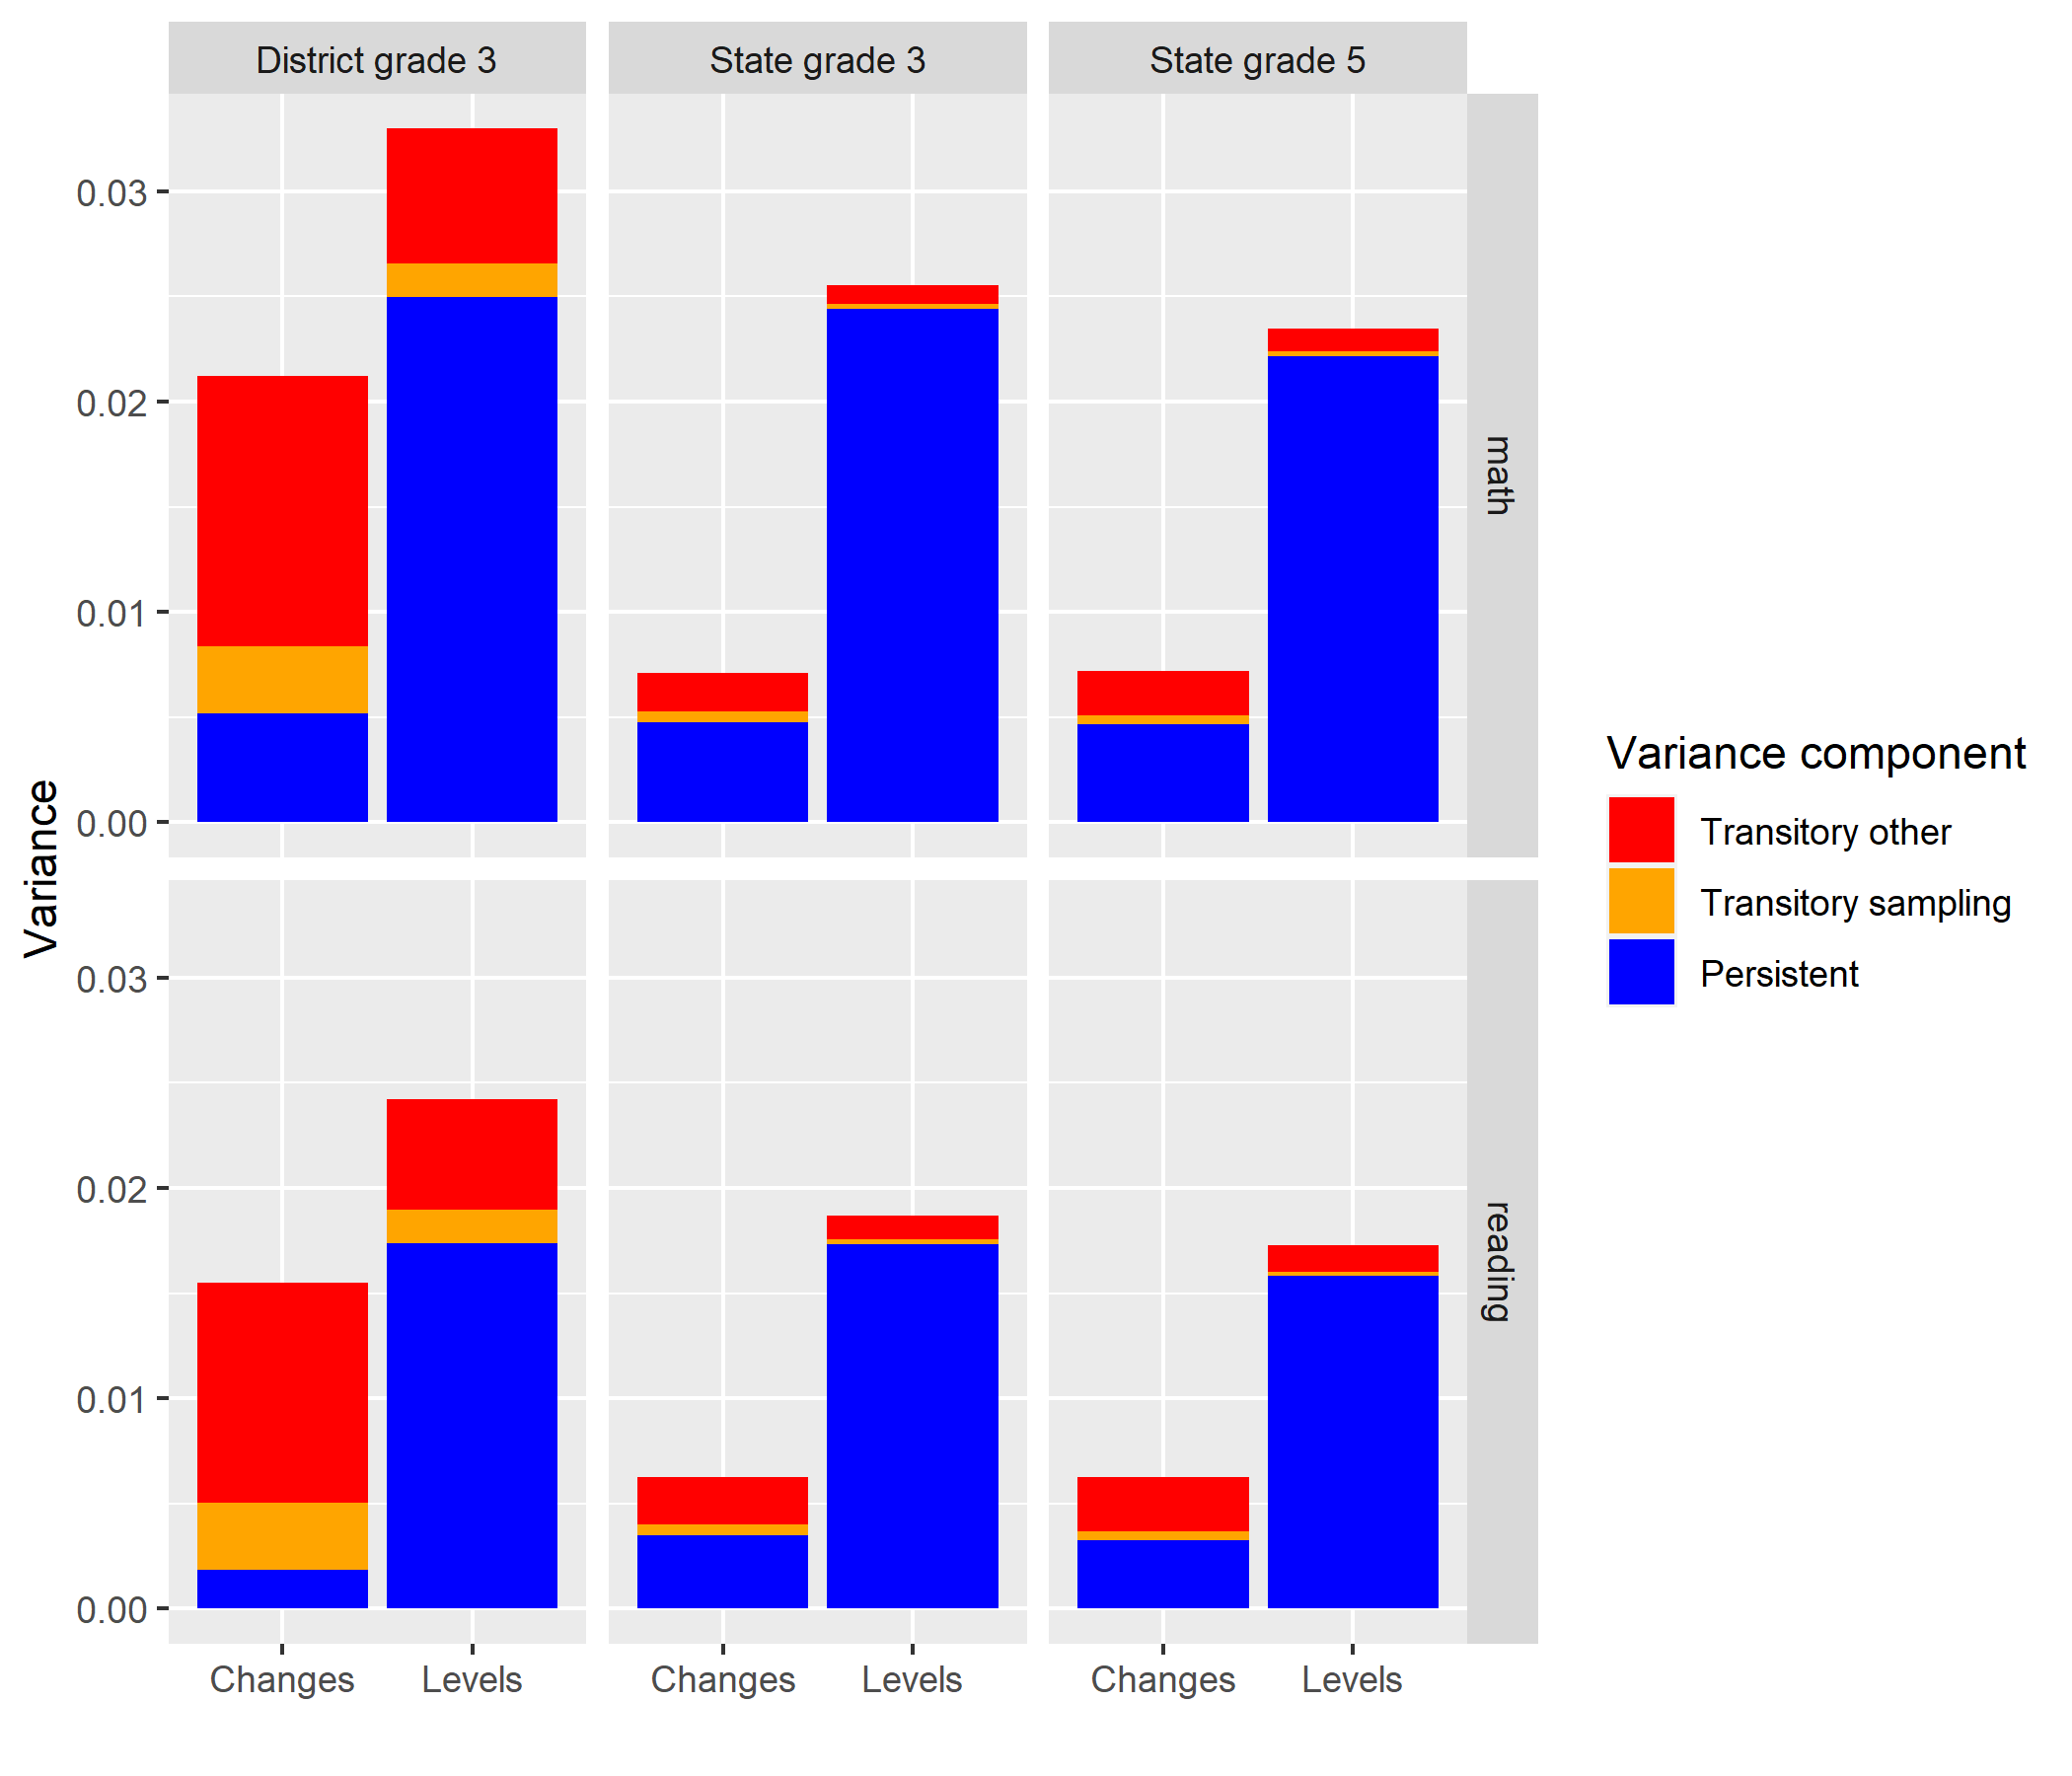
\includegraphics[width=0.9\linewidth]{Combined bar chart} 

}

\caption{Math Levels Over Time}\label{fig:combinedbarchart}
\end{figure}

For both reading and math, a large proportion (91\% to 95\%) of the variance in state scores (i.e.~levels) are due to persistent effects. The share of variance due to persistent effects is lower but still substantial for changes in state scores and district scores, ranging from 52\% for changes in state grade 5 reading scores to 76\% for grade 3 district math score levels. By contrast, the share of variance due to persistent effects is quite low for changes in district scores (24\% for math and 12\% for reading). For all subjects and aggregation levels and for both changes and levels, sampling variance makes up a relatively small share of overall variance and is much smaller than the variance due to other transitory effects.

Regressions of changes in class 5 state scores on twice lagged changes in grade 3 scores reveals that changes in grade 3 scores do not at all anticipate changes in grade 5 scores. The coefficient on twice lagged gains is -0.045 (std error = 0.069) for math and 0.036 (std error = .063) for reading. These results suggest that transitory effects are unlikely to be due to differences between cohorts.

If non-sampling transitory effects arise from survey error, these findings imply that comparisons between state levels based on ASER are relatively accurate but that comparisons between changes in state scores, districts, and changes in district scores will be less reliable. For example, taking grade 5 reading scores as an example, the variance decomposition implies that if we were to attempt to identify the top 25\% of states in terms of grade 5 reading scores, we would achieve roughly 75\% accuracy. By contrast, if we were to attempt to identify the top 25\% of states in terms of changes in
9 grade 5 reading scores, our accuracy would be only around 50\%.\footnote{These calculations assume that the two components are normally distributed though the results seem to hold for a variety of other distributions as well (including the \(\beta\) and t).}

\hypertarget{conclusion}{%
\section{Conclusion}\label{conclusion}}

We find that NAS state averages are much higher than ASER state averages and that NAS state rankings display almost no correlation with state rankings based on ASER, IHDS, or net state domestic product per capita. We conclude that NAS state averages are likely artificially high and contain little information about states' relative performance. Based on an analysis of internal reliability, we find that ASER data is mostly reliable for comparing state averages but less reliable for looking at changes in in state averages, district averages, or changes in district averages. Our findings have broad implications for how these existing data are used as well as potential future data collection efforts.

Our results for NAS suggest that NAS state averages (not to mention district results) should be used with extreme care if at all. Our results for ASER suggest that ASER is indeed a reliable guide for comparing state progress in basic literacy and numeracy but that care should be taken when comparing changes in indicators across states. Comparisons of changes in two states should be considered suggestive if the difference in their changes is small and rankings based on changes should be considered indicative. Researchers seeking to use ASER to estimate the impact of a policy may consider techniques which allow for error such as the methods described in Griliches and Hausman (\protect\hyperlink{ref-griliches1986errors}{1986}).

Taken together, these findings reveal a need for more precise data on learning outcomes in India. Data on learning outcomes for all children (those attending government and private schools in both rural and urban areas) with small standard errors at the state level would allow policymakers and the public to more accurately track progress in meetings the goals of the soon to be launched National Foundational Literacy and Numeracy Mission and researchers to more precisely estimate the impacts of education programs.

Our findings, along with other research in this space, also suggests ways to fill (or not fill) this gap. First, the disappointing results for the NAS data provide further evidence that collecting accurate data on learning outcomes, especially using assessments administered in schools, is exceptionally hard. Analysis of NAS training and guidance documents shows that much thought and care went into this exercise. For example, the method for randomly selecting students in classrooms, in our opinion, carefully balances the need for random selection with the need for practical feasibility. Our findings corroborate the evidence from Madhya Pradesh where Muralidharan and Singh show that scores on a set of assessments administered in schools were artificially inflated even though there were little to no consequences for having high/low scores (though they find that the assessments contained useful information about relative student/school performance) (Muralidharan and Singh \protect\hyperlink{ref-muralidharan2018improving}{2018}).

Second, we show that sampling variance accounts for a relatively small share (between one fourth and one ninth) of uncertainty in ASER state level estimates. This suggests that a survey with a smaller sample size but also less non-sampling variance could achieve similar levels of precision. For example, if a learning outcomes survey were to achieve zero non-sampling error it could attain ASER-levels of precision with only 1/16 to 1/81 the sample size (where we reduce sample size by reducing the number of villages rather than reducing students per village).

Taken together, this suggests that a smaller, household-based survey of learning outcomes using a tool similar to ASER but with more direct oversight and use of a full household listing for sampling may be a promising approach for collecting learning outcomes data. One option for such a survey would be to add on ASER to an existing household survey such as the one of the NSSO rounds or the NFHS. Such an approach would add very little marginal cost and the IHDS survey demonstrated the feasibility of adding an ASER-like tool to a large existing survey. Both NSSO and NFHS have well- developed internal systems for ensuring quality data collection. In addition, the rich set of additional household variables would allow for increased precision of district and state learning outcomes (through small area estimation and advanced imputation for missing assessment scores).

\newpage

\hypertarget{references}{%
\section{References}\label{references}}

\hypertarget{refs}{}
\leavevmode\hypertarget{ref-chay2005central}{}%
Chay, Kenneth Y, Patrick J McEwan, and Miguel Urquiola. 2005. ``The Central Role of Noise in Evaluating Interventions That Use Test Scores to Rank Schools.'' \emph{American Economic Review} 95 (4): 1237--58.

\leavevmode\hypertarget{ref-desai2015india}{}%
Desai, Sonalde, and Reeve Vanneman. 2015. \emph{India Human Development Survey-Ii (Ihds-Ii), 2011-12}. Inter-university Consortium for Political; Social Research Ann Arbor, MI.

\leavevmode\hypertarget{ref-filmer2018learning}{}%
Filmer, Deon, Margarita Langthaler, Robert Stehrer, and Thomas Vogel. 2018. ``Learning to Realize Education's Promise.'' \emph{World Development Report. The World Bank}.

\leavevmode\hypertarget{ref-griliches1986errors}{}%
Griliches, Zvi, and Jerry A Hausman. 1986. ``Errors in Variables in Panel Data.'' \emph{Journal of Econometrics} 31 (1): 93--118.

\leavevmode\hypertarget{ref-kane2002promise}{}%
Kane, Thomas J, and Douglas O Staiger. 2002. ``The Promise and Pitfalls of Using Imprecise School Accountability Measures.'' \emph{Journal of Economic Perspectives} 16 (4): 91--114.

\leavevmode\hypertarget{ref-kane2002volatility}{}%
Kane, Thomas J, Douglas O Staiger, David Grissmer, and Helen F Ladd. 2002. ``Volatility in School Test Scores: Implications for Test-Based Accountability Systems.'' \emph{Brookings Papers on Education Policy}, no. 5: 235--83.

\leavevmode\hypertarget{ref-muralidharan2018improving}{}%
Muralidharan, Karthik, and Abhijeet Singh. 2018. ``Improving Public Sector Management at Scale?''

\leavevmode\hypertarget{ref-aser2018}{}%
Pratham. 2018. \emph{Annual Status of Education Report (Rural)}. ASER Centre.

\leavevmode\hypertarget{ref-ramaswami2010survey}{}%
Ramaswami, Bharat, and Wilima Wadhwa. 2010. ``Survey Design and Precision of Aser Estimates.'' \emph{New Delhi: ASER Centre. Http://Img. Asercentre. Org/Docs/Aser\% 20survey/Technical\% 20Papers/Precisionofaserestimates\_ramaswami \_Wadhwa. Pdf}.

\leavevmode\hypertarget{ref-vagh2012validating}{}%
Vagh, Shaher Banu. 2012. ``Validating the Aser Testing Tools: Comparisons with Reading Fluency Measures and the Read India Measures.'' \emph{Unpublished Report. Retrieved July} 30.

\newpage

\hypertarget{appendix}{%
\section{Appendix}\label{appendix}}

\hypertarget{variance-decomposition}{%
\subsection{Variance Decomposition}\label{variance-decomposition}}

Figure \ref{fig:variance} below presents results from the analysis of ASER reliability using both the correlation decay method (our favored method) and the correlation in deltas method (our alternate method). Note that estimates of the share of variance due to sampling is the same across both methods.

\begin{figure}

{\centering 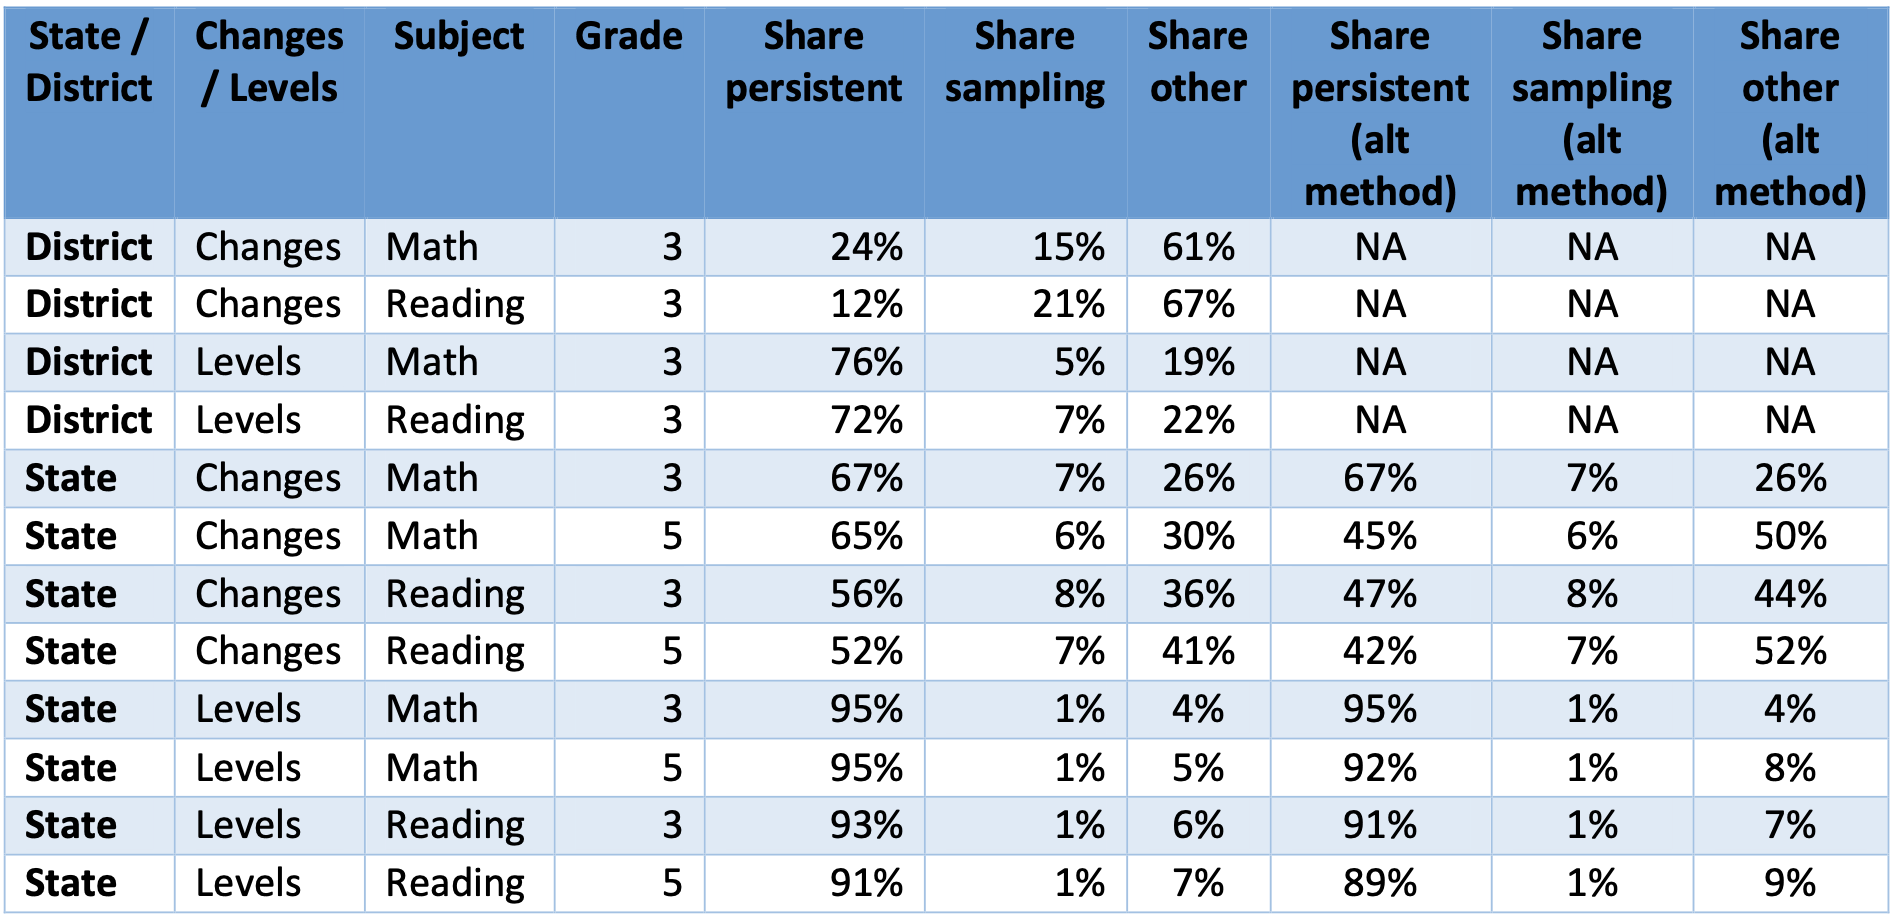
\includegraphics[width=0.8\linewidth]{variance_decomp} 

}

\caption{Variance Decomposition}\label{fig:variance}
\end{figure}

\end{document}
